\documentclass[dvips,12pt,a4paper]{report}
\usepackage[dvips]{graphicx}
\usepackage[latin1]{inputenc}
\usepackage[T1]{fontenc}
%\usepackage[portuges]{babel}
\usepackage[footnotesize]{caption}
\usepackage{subfigure}
\usepackage{amsmath}
\usepackage{amssymb}
\usepackage{bm}
\usepackage{lscape}
\usepackage{multicol}
\usepackage{longtable}
\usepackage{rotating}
\usepackage{color}
\usepackage{colortbl}
\usepackage{fancyheadings} % entete et bas de page
\usepackage{natbib}
\usepackage[left=3cm,right=2.5cm,top=3cm,bottom=3cm]{geometry}
\usepackage{setspace}
%\usepackage{natbib}
%\singlespacing
\onehalfspacing
%\doublespacing
%pour hautdepage
%[] page im paire {} page impaire
\lhead[\fancyplain{}{\sffamily \leftmark}]{}
\chead{}
\rhead[]{\fancyplain{}{\sffamily \rightmark}}
\cfoot{}
%\pagestyle{fancy}


%\usepackage{graphicx}
%\usepackage{txfonts}




\title{Abundances of refractory elements in exoplanet host stars}
\author{\\
\\
Vasco de Matos Ferreira Mendes Neves \\ [4mm]
\\
Department of Physics \\
University of Aveiro \\
Centro de Astrofisica da Universidade do Porto (CAUP) \\
University of Porto
\\
\\
\\
\\
\\
\\
\\
\\
Orientation by:\\
Alexandre Correia (UA) \\ Nuno Santos(CAUP)}
\date{June of 2008}

\begin{document}
\maketitle
%Abstract%%%%%%%%%%%%%%%%%%%%%%%%%%%
\begin{abstract}
 Aqui jaz o abstract. Ainda nao esta feito mas estara brevemente...no final...! Quando regressar aos ceus em toda a sua gloria...Que descanse em paz...por agora ;)
\end{abstract}
\newpage
\tableofcontents
\newpage


%Introduction%%%%%%%%%%%%%%%%%%%%%%%

\chapter{Introduction}
%\addcontentsline{toc}{chapter}{Introduction}

\section{In the Beginning...}

\indent\indent Since immemorial times man has asked himself if he was alone in the Universe. If there was life elsewhere beyond Earth. If there were other habitable planets in star systems orbiting other stars.

When the first exoplanet around a solar type star, 51 Peg, was discovered, by \citet{Mayor-1995}, %\textcolor {red} {when it's host star spectra was gathered after light years of relentless travel through the dark void among the stars}, 
a first, tiny piece of the huge puzzle that could answer these ages old questions was put into place. This discovery turned out to be one of the biggest breakthroughs in astrophysics of all times and sent shock waves that rippled through the teeming masses of humanity: there are other star systems in the Universe beyond our own...what next?

\indent Although this discovery and the others that followed shortly (e.g. \citeauthor{Marcy-1996} \citeyear{Marcy-1996}) had only detected giant planets with masses in the order of magnitude of Jupiter, the seed of possibilities had already been casted and the impact of these discoveries not only  opened a new field in astrophysics but also the minds and imagination of everyone. They have inspired passionate debates and, suddenly, old questions arrived renewed. Are there other earths orbiting other stars? Is life exclusive to Earth or is it common throughout the galaxy and the universe? Does this life, if it really exists, evolved and gained intelligence? And so on. 

Unfortunately, it does take endless hours of painstaking research and perseverance to reach for even the smallest answer. And then many more questions follow...that's how Science works! But let us now change subjects and move on to more pratical questions: the techniques that allowed the discovery of the explanet systems around solar type stars and their characterization.

%To conclude, we would like to suggest some reviews about the statistical results of exoplanet characteristics made by \citet{Udry-2007c} and \citet{Udry-2007}. - COLOCAR ISTO NA PARTE DAS PROPRIEDADES ESTATISTICAS

\section{The Radial Velocity Technique}

Those first discoveries, and most of the exoplanets that are found nowadays, are based in the Radial Velocity $(RV)$ technique. The use of this technique to detect planetary bodies was first proposed by \citet{Struve-1952}. It consists in the detection of the Doppler shift produced in the star's spectrum  by the subtle 'wobbling' of the star due to the presence of a planet in its orbit. If the star is moving toward Earth its light will be shifted to the 'blue' (i.e. the lines will move to shorter wavelengths). However, if the star is moving away from Earth its light will be red-shifted (i.e. the lines will move to longer wavelengths) as illustrated Fig. (\ref{rvpic}a). The radial velocity of the star can then be deduced from the displacement of the spectral lines. 
In Fig. (\ref{rvpic}b) we can see such variation depicting the orbital motion of a star. 

\begin{figure}[h]
\centering
\subfigure[]{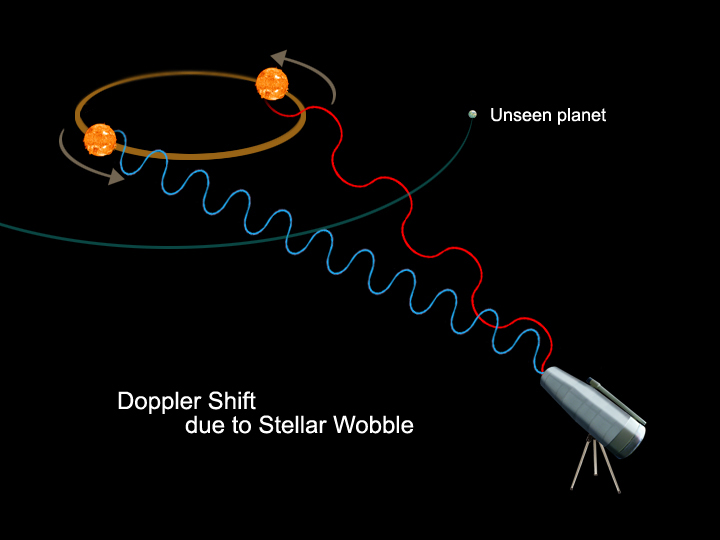
\includegraphics[height=6.3 cm]{pics/rvpic}}
\subfigure[]{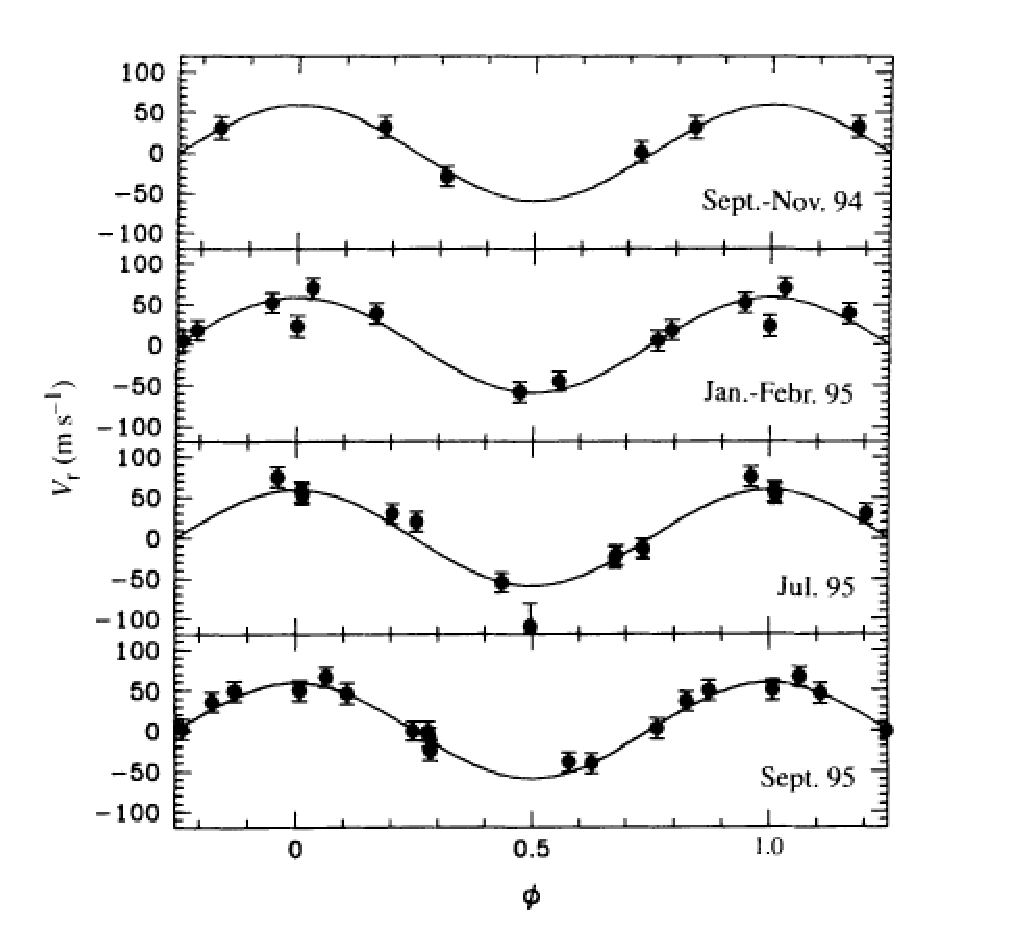
\includegraphics[height=6.3 cm]{pics/rv_1995}}
\caption[The RV Technique]{a) Illustration showing how the Radial Velocity technique works. Credits:www.nasa.gov ; b) Plots of radial velocity as funcion of the orbital phase, showing the orbital motion of 51 Peg at four different epochs \citep{Mayor-1995}}.
\label{rvpic}
\end{figure}

With the RV technique we can only ascertain with relative precision some orbital parameters (the semi major axis of the planet's orbit, eccentricity and orbital period) and a lower limit of the planet's mass. We cannot obtain the exact value of the mass because we lack the value of the inclination of the orbit of the planet to the line perpendicular to the line of sight. This fact is clearly expressed by the so called mass function,
\begin{equation}
 f(m)=\frac{(msini)^3}{(M+m)^2}=1.036.10^{-7}K^2(1-e)^{3/2}P\,\,\, [M_\odot]
\label {vradial}
\end{equation}
where $m$ is the planet's mass, $i$ is the inclination, $M$ is the star's mass, $e$ is the eccentricity, $K$ is the measured semi-amplitude of the radial velocity, $P$ is the measured period of the star's wobble (that is equal to the planet orbital period around the star) and $G$ is the gravitational constant. The $P$, $e$ and $K$ can be directly obtained from the RV curve. The $msini$ is then calculated with this equation. For a detailed demonstration refer to (Santos 2008). From Eq. (\ref{vradial}) we can clearly see that the amplitude of the radial velocity will be greater if the planet is closer and/or is more massive. This means that planets with smaller masses and further away from the star will be more difficult do detect. 

The $RV$ technique does not give us the atributes for the planet radius and is unsuitable to detect planets in stars that are too massive, are instable or rotate too rapidly. Therefore, the detection of planets with it is restricted to 'quiet' FGKM dwarf stars. If we want to acquire the radius and, with it, the mean density of the star, we need to use other techniques such as photometric transits or astrometry and combine the data of the two methods.

Nevertheless, the RV technique is far from having reached his highest point: It is expected that the precision can reach a limit of $1cm/s$, enabling the detection of sub earth planets \citep{Lovis-2006b}. 


%Using Kepler's third law, the period of the planet's orbit around a star (that is equal to the variation of the star's wobble) can be used to determine the distance of the planet to the star, 
%\begin{equation}
% r^3=\frac{GM_{star}}{4\pi^2}P_{star}^2,
%\end{equation}
%where $r$ is the radius of the planet, $G$ the gravitational constant, $M_{star}$ the mass of the star and %$P_{star}$ the observed period of the star's wobble.

%The mass limit is due to the unknown value of the inclination of the orbit of the planet relative to the star, [ver %wikidopplerspectroscopy]
%\begin {equation}
%\label {eq 1.1}
%M_{p}=
%\end {equation}
%, where $M_{pl}$ is the planet's Mass, 

\section{Photometric Transit Technique}
\label{transit}
A photometric transit occurs when a planet crosses in front of the star and blocks part of its light. 
The photometric transit technique consists in the measurement of the variation of the star's brightness at the moment of the transit. When a planet crosses in front of the star, the star brightness will drop by a small amount. For a Jupiter like planet, this variation is of the order of 1\% and for less massive planets is even smaller citep{Santos 2008}. 

This technique can only detect orbits of planets closely aligned with earth. The estimated probability that a full transit will happen is given by the geometric probability, $P=R_{star}/a$, where $_R{star}$ and $a$ are the stellar and orbital radius, respectively. This is only valid for circular orbits. While the probability of detecting a planet with $P=3$ days is about 10\%, it goes down to 0.5\% for a planet orbiting 1 AU from its star.

Another disadvantage is related its high rate of false detections, where changes in the brightness of the star are provoked by other fenomena such as eclipsing binaries, grazing stellar eclipses or variations in the chromospheric activity (false detections) \textcolor{red}{confirmar} . Therefore, the only way to be sure is to do a follow up with $RV$. 

The greatest advantage of the transit technique is that we can determine the radius of the planet from the light-curve. We can see an example of a phototransit event in Fig. (\ref{photot}a). 

\begin{figure}[h]
\centering
\subfigure[]{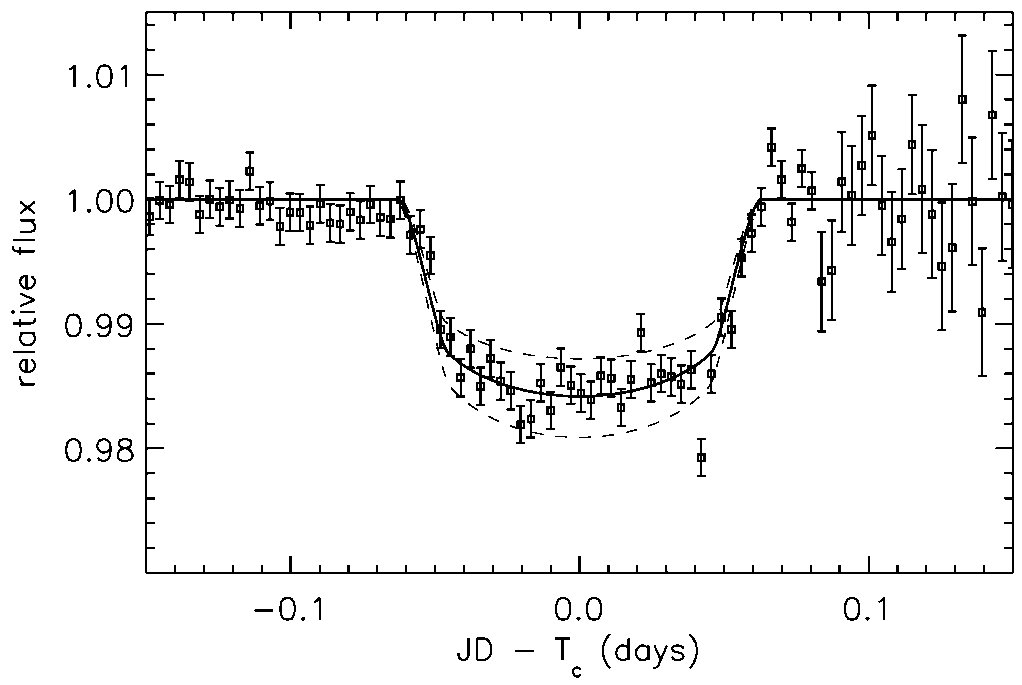
\includegraphics[height=5 cm]{pics/phototransit}}
\subfigure[]{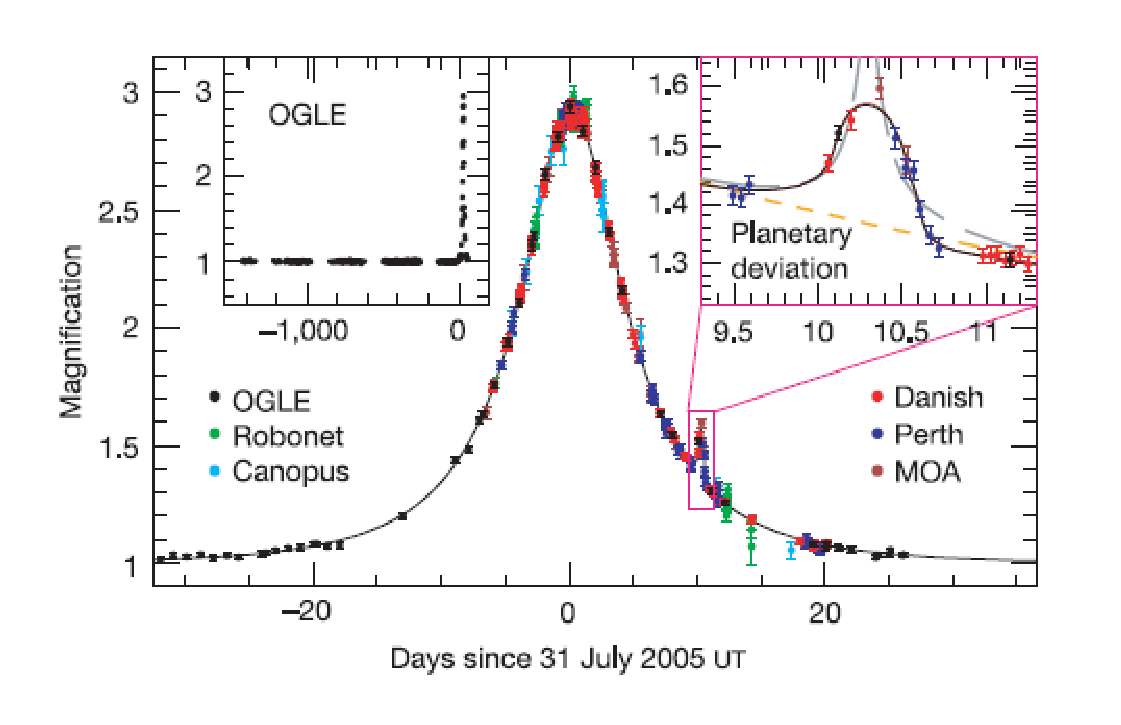
\includegraphics[height=5 cm]{pics/microlensing2}}
\caption[Example of a phototransit and microlensing event]{a) Photometric time series, binned into 5 minute averages. The solid line represents the best fit for data. The dashed lines represent transit curves if the transit planet had $\pm10\%$ in size. From \citet{Charbonneau-2000}; b) Observed light curve of the OGLE-2005-BLG-390 microlensing event and best-fit model plotted as a function of time. From \citet{Beaulieu-2006}.}
\label{photot}
\end{figure}

If we combine the information obtained in $RV$ with the one obtained in a photometric transit \citep{Charbonneau-2000}, we can determine the exact mass and density of the planet and estimate its composition.

It is also possible to study the chemical abundances of a transitign planet's atmosphere by comparing the spectra of its star before and during the transit. The first detection of the signature of Sodium in HD 209458b, a hot Jupiter, was accomplished by \citet{Charbonneau-2002}, and the signature of Carbon and Oxygen was discovered in the same planet by \citet{Vidal-Madjar-2004}. Both groups used the HST to make the detections.

The future of the transit technique is most promising: today dozens of surveys are made and the possiblity to study the density and atmospheric composition of the planets is within reach. Higher expectations came from the space based missions, both present (COROT) and future (Kepler): they may allow the detection of earth size or even smaller planets. In conjunction with $RV$ it will be possible to study 'Earth domain' mass-radius relation.

\section{Astrometry}
\label{astrometry}
Astrometry is the oldest searching method for detecting extrasolar planets but not the most effective (yet). It consists in the very precise measuring of a star's position over time. The presence of another sufficiently orbiting massive body, will make the detection of the star's motion around the center of mass of the system possible. Only recently the first detection of an exoplanet with this method was possible \citep{Benedict-2002}, using the HST. 

Unfortunately, current astrometric technology does not allow the detection of planetary bodies from scratch: up to now, all detections made with astrometry were follow-ups to successfull measurements by RV. It will be needed to surpass the 1 micro-arc-second threshhold for an independent and reliable detection of planetary bodies with astrometry.

In conjunction with $RV$, it gives the exact mass of the planet, along with astrometric parameters (perturbation of the semimajor axis, inclination and absolute parallax). Astrometry is also complementary of the $RV$ in the sense that it is more sensitive to longer period planets. On the top of that, it enables the detection of companions in stars where $RV$ is impraticable: A,B stars and T-Tauri stars.

\textcolor{red}{sera q devo incluir aqui as equacoes e explicar as desvantagens (q estao intrinsecamente ligadas) ou pode ficar assim?}

Regarding astrometry, HST, JSWT (the space missions), VLTI and the Kech Interfermoter will enable the gathering of astrometric parameters of the planetary systems and allow the determination of the exact mass of the planetary companions. Further in the future, the space missions GAIA and SIM will, hopefully, detect thousants of planets by pushing the detection limits towards sub earth mass planets.



\section{Microlensing} 
\label{microlens}
\indent In this context we should not forget the role of a promising technique, microlensing \citep{Beaulieu-2006}, also very complementary of $RV$, with the potential of detecting sub earth mass bodies in long orbits and at a much larger distance of detection (up to 10kPc). Microlensing occurs when the gravitational field of a star acts like a lens, magnifying the light from distant stars. If the star that provokes the lensing has a planet, then the planet's field can make a detectable contribution. One example can be seen in Fig. (\ref{photot}b). We can estimate the mass, period and semi major axis of the planet with this method. However, it has a great disadvantage: the lensing is difficult to reproduce because the chance alignment may never occur again. Moreover, the detection of the more distant planets is impossible to confirm  by other methods (i.e. RV, Astrometry).
\\
\\
All methods of planetary detection past and future, along with future ground and space based missions can be reviewed in \citet{Perryman-2005}. - \textcolor{red}{METER N SEI ONDE}



%Considering the stellar properties, further studies on metallicity will be conducted on the new found systems. It will be most interesting to see how the trends in metal poor stars and solar system similars will develop. - VAI PARA A PARTE DOS METAIS



%\section {Spectra from other worlds - removido} 

%\indent Against all expectations, the transit technique also allowed the first detection of the signature of Sodium, Carbon and Oxygen in HD 209458b, a hot Jupiter, with the Hubble Space Telescope $(HST)$ \textcolor{green}{(Charbonneau et al 2002)}. In 2007, it was discovered the first clear sign of water vapor, also on a hot Jupiter, HD 189733b \textcolor{green}{(Tinetti et al (nature VER))}. The detection of methane followed a few months ago \textcolor{green}{[referencia...]}. This means that we can now detect some elements that are precursors of life as we know it...the firsts steps towards detecting life in another world. 

%However, the discovery sought by all is an earth type planet capable of supporting life. The smallest planet yet discovered is GJ 581c \textcolor{green}{(Udry et al. (2007))} with a minimum mass of 5 earth masses and a estimated radius of 1.5 earth radius. This planet was detected by $RV$ and it's on the limit of the detection. But that's not all: this 'super-earth' resides inside the habitable zone of that star. It would be of great interest to detect a transit of this world in order to acquire his spectra. Nevertheless, we will have more data regarding this and other interesting planets very soon, with the upcoming ground and space missions \textcolor{green}{(see Perryman et al. 2005)}.

\section {A statistical 'zoo' of exoplanets}

\indent Up to now, and according to the `The Extrasolar Planets Encyclopaedia', there are 287 planet candidates detected in 248 planetary systems, which gives 27 multi planet systems (http://www.exoplanet.eu/catalog.php). The system with the greatest number of planetary bodies found, for now, is 55 Cancri, with 5 planets \citep{Fischer-2008} and the smallest planet yet discovered (by $RV$ with HARPS - precision ~ $1m/s$) is GJ 581c \citep{Udry-2007b} with a minimum mass of 5 earth masses and a estimated radius of 1.5 earth radius. 

Looking all this data, we can admire the real 'zoo' that exoplanets became: Orbiting stars of spectral types from F to M, we get minimum masses from $5 M_{\oplus}$ to 20 $M_J$, periods from a little more of 1 day to 5218 days and eccentricities from perfect circular orbits to extreme values of more than 0.90. There are planets as close as $0.0177 AU$ and as far as $670 AU$ from its host star.

This information can be of great help in setting constraints to planetary formation, internal structure and atmosphere models. With this in mind, we can analyse the distributions of the eccentricities, periods and planetary masses and we try to relate them among each other and with another measured parameters like the host star properties (chemical composition, effective temperature, surface gravity, mass, age). For instance, in Fig (\ref{planetmass}) we can see the Period-Mass distribution of known extrasolar planets orbiting solar type stars.

\begin{figure}[h]
\centering
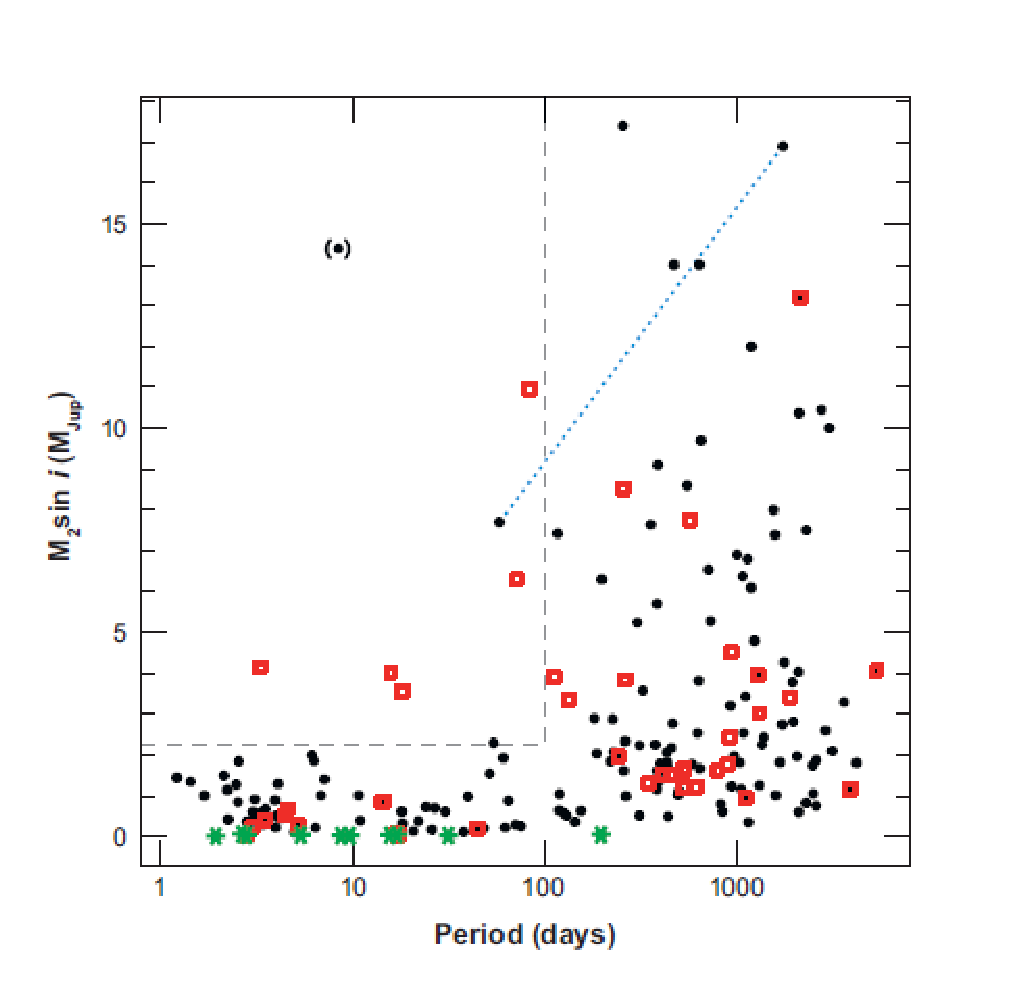
\includegraphics[height=10 cm]{pics/massplanet2}
\caption[Period Mass distributions of known extrasolar planets ]{Plot of Period-Mass distribution of known exoplanets orbiting solar type stars. The black dots, red squares and green stars represent planets around single stars, planets in binaries and solid planets, respectively. The gray dashed lines represent a limit at 2.25 $M_{jup}$ and 100 days. The blue dotted line connects the two massive bodies orbiting HD 168433. The parentheses indicate the position of the probable brown dwarf HD 162020 \citep{Udry-2007}. }
\label{planetmass}
\end{figure}

We can clearly observe that there is a lack of massive planets in short orbits. If we exclude multiple systems we can see that there is no planet larger that 2 $M_{jup}$ at all in orbits shorter than 100 days. This might be a consequence of a migration process or a mass transfer (or even absorption) of the planet into the star \citep[e.g.][]{Trilling-1998}. %Another interesting aspect is the fact that massive planets prefer to reside farther from the star. This can be explained by the fact that they have more planetesimals to aggregate along a longer orbit. Thus they can grow more \citep{Pollack-1996}. Then, they tend to became 'stranded' due to their larger size and lack of enough material to overcome their inercia.
 
\section {The formation of planetary systems}
\label {planets}
\indent Despite all this bounty of data, we still have a cloudy view of the physical mechanisms behind the formation of planetary systems. The appearance of giant planets close to the star and the existence of bodies with high eccentricity completely changed the way simulations were made. Quite simply, these cases never appeared in the computational models because the constraints used in the possible scenarios were based only on our solar system...

Nowadays, there are two major theories about the formation of exoplanets: core accretion and direct gravitational instability. 

The first one tells us that planets are formed via accretion of dust grains due to gravity. They continuously grow and collide with each other until they formed planetesimals, with a few kilometers in diameter. These bodies continue to grow and collide until they reach bigger sizes, over the course of a few million years. If the mass of a protoplanet reaches 10 to 15 $M_{\oplus}$ before the dispersion of the disk of gas, a runaway accretion will follow and a gas giant will form. On the contrary, if the mass doesn't reach the critical value necessary for runaway accretion, a smaller rocky planet or Neptune type gas planets will form (\citeauthor{Pollack-1996} \citeyear{Pollack-1996}; \citeauthor{Alibert-2006} \citeyear{Alibert-2006}). 

The second one states that planets form by disk instability: the solar nebula breaks up, through its own self gravity, into clumps of gas and dust, rapidly forming protoplanetary bodies. They are expected to be massive gas giants, forming really fast ($~10^3$ years compared to the accretion $~10^6$ years in an optimistic scenario) \citep{Boss-1997}. 

The planets could then migrate or remain more or less in the location of formation. This will depend mainly on planet-disk interactions \citep{Trilling-1998}.

The metallicity also seems to play an importante role. This will be shown in more detail in subsection \ref{metal}

\section{The host star properties}

In this section, we will discuss the properties of the planet host stars (chemical composition, mass, age, rotation) and their correlations. As we will see, these properties are providing important clues about the formation of planetary systems and its constraints.

\subsection {The Metallicity Distribution} 
\label{metal}
The vast majority of the host star's analysis are of spectroscopic nature and are based mostly on iron abundances. These have revealed that a giant planet have a much higher probability of forming when its host star has, on average, a greater metallicity than of its neighbours, at least for [Fe/H] above the solar value (e.g. \citet{Gonzalez-1998}, \citet{Gonzalez-2001}, \citet{Laws-2003}, \citeauthor{Santos-2001a} (\citeyear{Santos-2001b}, \citeyear{Santos-2001a}, \citeyear{Santos-2003}, \citeyear{Santos-2004b}, \citeyear{Santos-2005a}) , \citet{Fischer-2005}. It was also shown that this result is not biased  (e.g. \citeauthor{Santos-2003} (\citeyear{Santos-20	03}, \citeyear{Santos-2004b}), \citet{Fischer-2005}). This means that metallicity has a crucial role in the formation and evolution of planets (or at least the giant ones). Interestingly enough, it seems that, for low metallicities, the frequency of planets may remain constant \citep{Santos-2004b}. In Fig. (\ref{histfeh}) we can see two histograms of the frequency of planet hosts in function of [Fe/H], where this behaviour is evident. 

\begin{figure}[h]
\centering
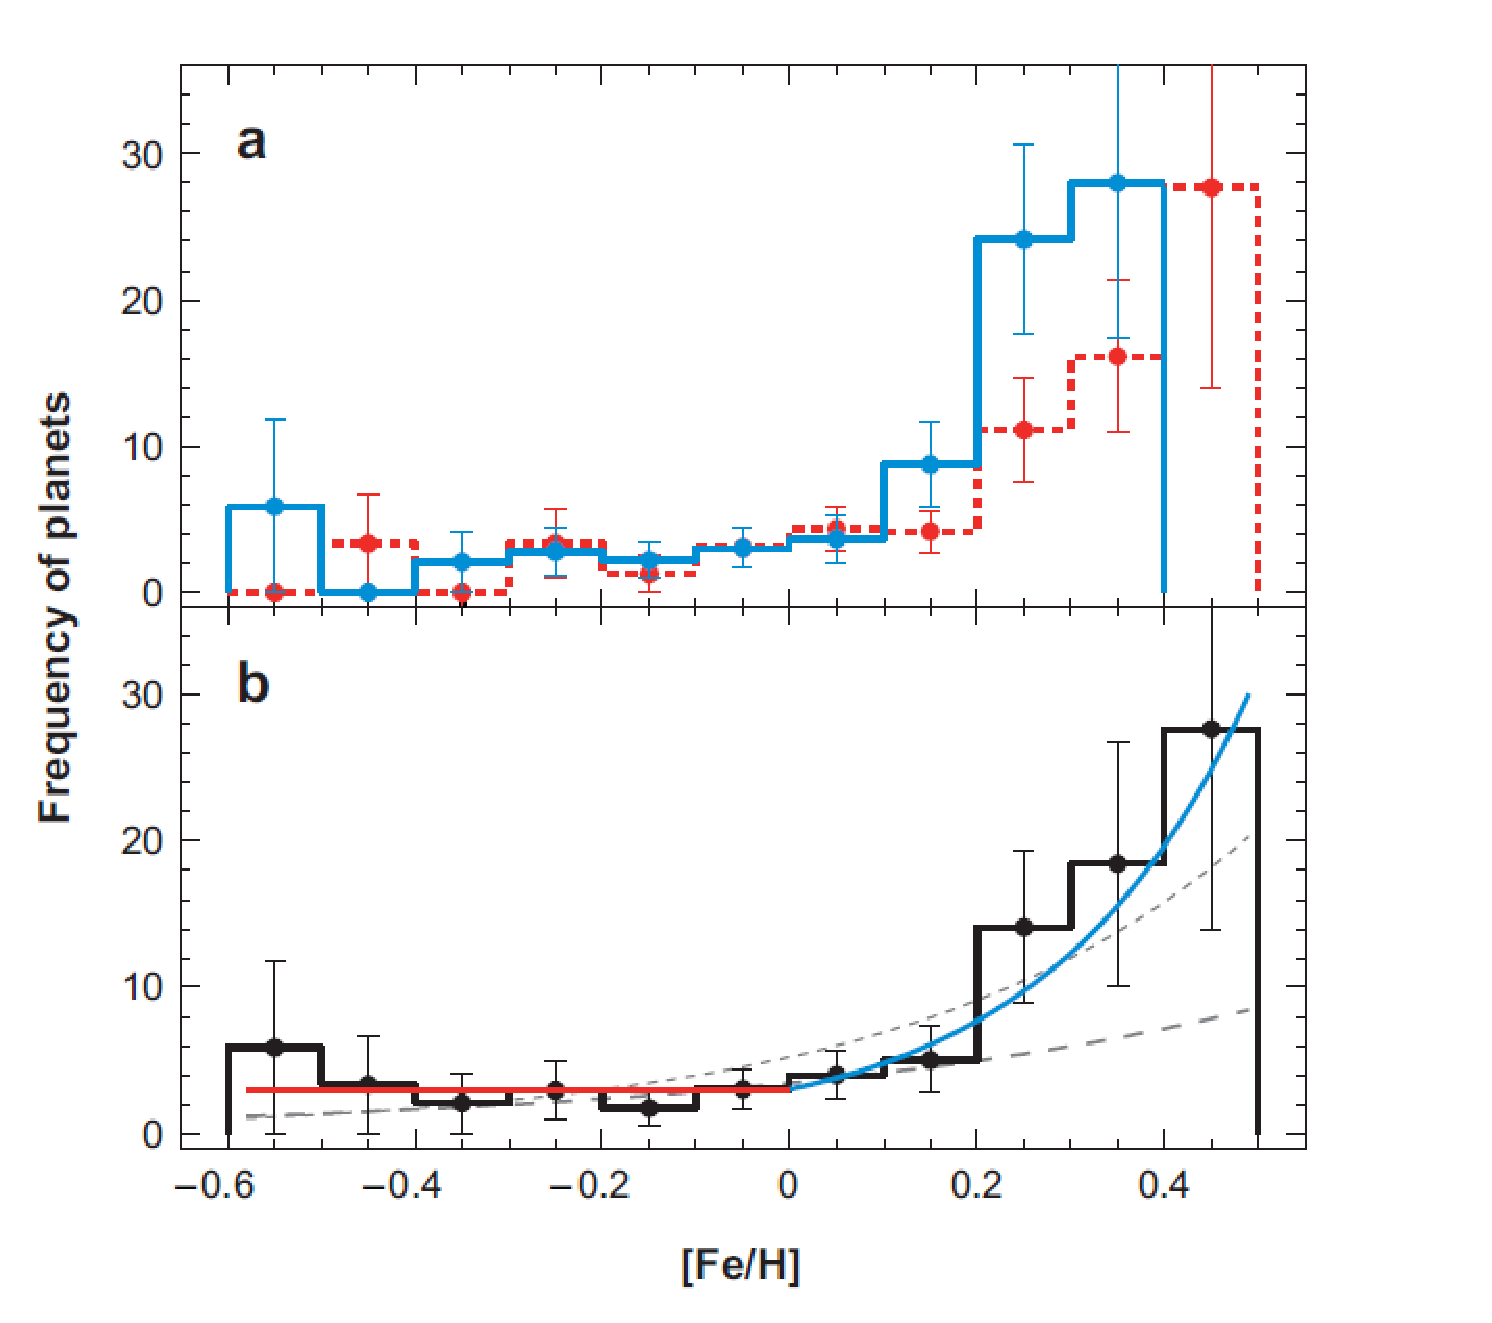
\includegraphics[height=10 cm]{pics/fehhist}
\caption[Histograms of Frequency of planets with metallicty ]{a) Percentage of planet hosts as a function of stellar metallicity from CORALIE (blue) and Lick-Keck (red) samples. The lowest metallicity part of the histogram has few planet hosts and therefore its statistics are poor.; b) Average distribution of the two samples. The blue curve represents a power law fit of the data using only the [Fe/H] values greater than 0.0. The red line represents an average value for [Fe/H] between -0.5 and 0.0.  \citep{Udry-2007}.}
\label{histfeh}
\end{figure}

For neptune class planets no such trend is observed. However, there aren't enough planets yet to make a sound statistical distribution \citep{Udry-2006}.

Shortly after this crucial observation, two different hypothesis for this 'anomalous' metallicity arose: the primordial origin and the external pollution process. 

The first one defends that the high metal content of the star originated from the primordial cloud that gave origin to the star system. The detected metallicity is seen as nothing more than a consequence of gallactic chemical evolution. The host star planets are simply in the high mettalicity end of the distribution. This scenario was favoured in recent studies (\textcolor{green}{(e.g. Santos et al 2001a,b,2003,...inda n esta feito)}. 

The second one posits that the high metallicity found in some stars is due to the late accretion of planetary material. Some evidence was found for this latter scenario: hints of pollution were discovered by \citet{Gonzalez-1998} in 16 Cyg  in the form of an iron enhancement. However, \citet{Santos-2001b} had noticed that the quantity of material that is needed to change a star's iron content is much bigger than the one that was detected, especially if we consider pollution as the dominant factor in the determination of a star's metallicity. 

These two mechanisms leave different imprints: in the former case the star formed in a high mettalicity cloud will always be metal rich; in the latter case, the high metallicity is confined to the star's convective zone but its interior is left metal poor. In this context, it's important to emphasize that F dwarfs with relatively thin convective zones will exhibit a greater degree of pollution \citep{Fischer-2005}. Therefore, the upper part of the distribution of metal abundance of a F dwarf should exceed the highest value of G dwarfs, but it doesn't. On the other hand, this pollution will dillute with the passage of time, mixing with deeper, unenriched layers. Moreover, giant stars with planets, despite having a much larger convective envelopes, do not present a lower metallicity when compared to planet host stars similar to the sun \citep{Ecuvillon-2006b}. A study on the abundances of elements other than iron might give us clues on this important question (see subsection \ref{others}).

It is true that pollution can be important in a few isolated cases. However, the most accepted view today is that pollution has a small part in the global metallicity of the star but it's not the dominant process. 

\subsubsection {Implications for planetary formation theory}

As we have seen in Section (\ref {planets}), there are two main models of planetary formation: core accretion and gravitational instability. The former predicts that the efficiency of planetary formation depends on mettalicity. The latter doesn't. The fact that the proabability of finding a giant planet increases with [Fe/H] thus favours the core accretion model. This dependence can even be predicted by current models \citep{Ida-2004a}. However, it is not known how an increase in the metallicity will change the parameters that reign over the formation and evolution of planets. The inability to use one single power law to fit the distribution of Fig. (\ref{histfeh}b) might suggest that there are two regimes of planetary formation.


%These results may have important consequences in the constraining of the parameters for the computational models of planetary systems (\citet{Pollack-1996}, \citet{Boss-2002}).

\subsection {Abundances of other elements} %***
\label {others}

For some time, the studies of metallicity were restricted to Iron. Then, works on the abundance of other elements gradually started to appear.
Many studies were made to analyze the abundances of light elements (e.g. \citet{Israelian-2003}, \citet{Sandquist-2002} and other elements {(e.g. \citet{Gonzalez-2001}, \citet{Fischer-2005}, \citet{Takeda-2001}, \citet{Ecuvillon-2004b}. Refractory elements were also analysed by e.g. \citet{Bodaghee-2003} and \citet{Gilli-2006} (...). Na, Mg and Al were investigated by \citet{Beirao-2005}. 

Some interesting tendencies were found out. In the study of the origin of the high mettalicity of planet host stars, for example, \citet{Israelian-2003} found out that HD 82943 had a significant amount of $^6Li$ in its stellar spectrum. This is only possible if the star had engulfed lots of planetary material, because almost all $^6Li$ is destroyed before the star enters in the main sequence and should not be detected \citep{Sandquist-2002}. Therefore, this evidence favours the accrection of planetary materials scenario (see subsection \ref{metal}). Hints of pollution were also found by \citet{Laws-2001} in 16 Cyg  in the form of a lithium enhancement.

However, \citet{Ecuvillon-2006b} showed that there is no increase in [X/H] with the condensation temperature for volatile and refractive elements, contrary to what was expected if pollution was the main cause of the metallicity excess (i.e. volatiles of the planet should evaporate before the accretion takes place). 

Despite that, it's worth noting the strange behaviour of [X/Fe] of some elements (eg Mg,Mn,V,Co) on planet host stars (\citet{Bodaghee-2003},\citet{Gilli-2006}) . This is very difficult to explain by gallactic chemical evolution but these differences might be related to NLTE effects \citep{Bodaghee-2003}.

But, on the top of that, it was shown once again, this time for other elements, that the frequency of giant plants is a strong function of the metallicity of its host star (e.g. \citet{Fischer-2005}, \citet{Gilli-2006} (...). It seems that the high metallicity enhances the formation of planets because, quite simply, there's more material to aggregate.

. %The last two studies required a uniform high metalicity comparison field sample, because they lacked single stars with Fe/H values higher than 0.1.  - por parte 3 %This was achieved by Gilli et al. (2006) that also provided new results using high quality spectra from a group with 101 planet host stars and 93 stars with no known planetary companions, in a uniform metallicity range between -0.7 and 0.45.  - por parte 3.

%As we can see, some studies revealed a few possible but unclear anomalies. In our study, with the high precision spectra, we will try and see if those anomalies are just bad data or if there is more than that. We will directly compare our results to this paper as we will see later on.   \textcolor{red}{[Falar no problema dos erros sistematicos na parte 2 devido as amostras de comparacao inomogeneas - source of systematic errors!!!]}

%Is is known that light elements such as $Li$ and $Be$ can be very important tracers of the history of solar type stars and therefore can be used to distinguish between different planet formation scenarios (Sandquist et al 2002). These light elements, as well as others, volatile and refractory, can also give us hints about pollution in the chemical composition of a star, if an excessive abundance of $_6Li$ or the ratio $_6Li$/$_7Li$ is detected (ver referencia!!! Sandquist?) or if an overabundance of refractory elements over volatile is observed. However the results obtained are not conclusive (Ecuvillon et al 2006) in detecting anomalies in elemental abundances or hints of pollution.

\subsection {Correlations between metallicity and orbital parameters}

The possible correlation between metallicity and orbital parameters has been studied. (e.g. \citet{Gonzalez-1998}; \citet{Santos-2003}; \citet {Fischer-2005}). No clear correlation has surfaced. However, stars with short period planets seem to be particularly metal rich. \citet{Ida-2004b}, in their work of planetary formation modelling, have shown that a higher metallicity allows a faster or/and closer formation of giant planets closer to their host star. Therefore, the planets have more time to migrate, and this could explain the fragile correlation.  On the other hand, if the migration if fast enough, this correlation has little meaning.

\subsection {The host star mass}

The relation of stellar mass with planetary frequency has been explored \citep{Laws-2003}. It seems to exist a slight tendency for a greater frequency of planets in stars with mass up to  1.5 $M_\odot$. Any possible conclusion is greatly limited by the fact that radial velocity studies are restricted to the mass range between 0.7 to 1.5 $M_\odot$. 

\citet{Burkert-2007} have studied the relation between stellar mass and planetary orbital periods. They discuss that the observed shortage of massive planets in semimajor axes in the range 0.1-0.6 AU may result from a gap in the modelled radial distribution of planets. This gap may be due to shorter depletion timescales (that imply an early stop of migration) or to strong UV radiation in the early stages of planetary formation (pre main sequence).

More studies are needed to adress these and other issues concerning the host star's mass and its relation with planetary parameters.

\subsection {Other correlations}

Many other correlations have been explored: for instance, the relation between the presence of planets and chromospheric activity levels, ages and rotational periods of stars. No clear relations were found. However these studies are limited and possibly biased due to the fact that the stars observed are from a restricted sample ('quiet' FGK stars). Again it is necessary more research. For an overview see  \citet{Udry-2007}.

%\subsection {Our work - this sucks...}

%Following the studies made for the abundance of Iron and for other elements we will make, on this work, a detailed statistical analysis of the abundances based on a subsample of the HARPS GTO planet search program containing 451 stars. Of these, 66 are planet hosts and the other 385 stars are dwarfs with no known planet. In the following chapters we will present a detailed analysis of all the steps in obtaining the abundances of all the elements studied, followed by the discussion and interpretation of the results obtained.

\section{Objectives isto inda n ta feito}

This objectives of this work are as follows:
\begin{itemize}
\item Identification and selection of spectral lines for each species.
\item Spectroscopic Analysis of the 
\item 
\end{itemize}


%%%%%%%%%%%%%%%%%%%%%%%%%%%%%%%%%%%%%%%%%%%
%CHAPTER 2 %%%%%%%%%%%%%%%%%%%%%%%%%%%%%%%%%
%%%%%%%%%%%%%%%%%%%%%%%%%%%%%%%%%%%%%%%%%%%%%

\chapter{Determination of Chemical Abundances}

\indent In this chapter, we will present a brief outlook on the determination of chemical abundances from spectral lines. For a more profound insight refer (especially) to chapter 13 (The Behaviour of Spectral Lines) and 16 (Chemical Analysis) of \citet{Gray-2005}. All pictures are taken from this book except when said otherwise.

If we take a good look at a regular stellar spectra we can easily identify the presence of many elements. They are there in the form of absorption lines. These lines correspond to electronic transitions among the different levels of its atoms (bound-bound transitions). This is especially true for cooler stars of the FGKM end of the HR diagram,where the atoms and molecules of many species are not fully ionized. In general, the results of chemical analysis show us that hidrogen is the most abundant element (~90\%) in the stellar photosphere, followed by helium (~10\%). The remaining elements, refered as 'metals', only account for a tiny percentage of the abundance. However, most spectral lines have origin in metal species.

These lines show different shapes and strengths that derive directly from the conditions in the photosphere of the star (temperature, pressure, radiation, magnetic and velocity fields). We do not yet know how to totally 'deconvolute' this factors, but we will try to separate the effect of chemical composition from the other factors as much as possible. In spite of that, the most important aspect in the determination of an element's abundance is that the strength of line absorption depends on the number of absorbers that correspond to that transition. 
%Therefore, the calculation of the atomic level populations are very important in the calculation of the abundance.

Chemical composition can also give us insight of many phenomena (nuclear reactions, dynamics, accretion of materials in stars; light elements (Li, Be,C) as tracers of evolucionary stages of the star; the galactic chemical evolution). 

\section {Local Termodynamic Equilibrium}
\label{LTE}
If we consider that collisions (rather that radiation) dominate the excitation of the atoms (as in the case of Sun type stars), then local thermodynamic equilibrium (LTE) will apply and  \textcolor{red}{confirmar!} we can express the ratio between the number of atoms per unit volume in a level $n$ and all the atoms of that species as
%\begin{equation}
%\frac{N_u}{N_l}=\frac{g_u}{g_l}e^{-\Delta\chi/kT},
%\label{Boltz}
%\end{equation}
\begin{equation}
\label{Boltz}
 \frac{N_n}{N}=\frac{g_n}{u(T)}10^{-\theta(T)\chi_n},
\end{equation}
where $N_n$ is the population of level $n$, $N$ is the total number of atoms, $g_n$ is the degenerency of level $n$, $\chi_n$ is the energy of the same level, $\theta(T)=\log(e)/(kT)$, $u(T)=\Sigma g_ie^{-\chi_i/kT}$ is the partition function, $k$ is the Boltzmann's constant and $T$ is the temperature. This is one formulation of the well known Boltzmann equation. %Note that $k$ must come in units of $eV/K$ in order to be compatible with $\chi$ in $eV$.

Similarly, the ionization for the collision dominated gas can be calculated using Saha's Equation,
\begin{equation}
\label{Saha}
\frac{N_1}{N_0}=\frac{\Phi(T)}{P_e},
\end{equation}
where 
\begin {equation}
\Phi(T)=\frac{(\pi m_e)^{3/2}(2kT)^{5/2}}{h^3}\frac{u_1(T)}{u_0(T)}e^{-I/kT}.
\end {equation}
The $N_1/N_0$ is the ratio of ions to neutral atoms, $u_1/u_0$ is the ratio of ionic to neutral partition functions, $m_e$ is the electron mass, $h$ is the Plank's constant, $P_e$ is the electron pressure and $I$ is the ionization potential.

The Eqs. (\ref{Boltz}) and (\ref{Saha}) represent the physical processes behind the abundances of the different elements. In section (\ref{calab}), we will see how the calculation of the abundance is made.

\subsection {Computing the line profile}

\indent If we have an equilibrium situation, for each emitted photon there must be another that is absorbed, and a line will form. This is the case in LTE. As we will see in the following sections, LTE will be used to calculate our model atmosphere \textcolor{red}{(verificar)} and help us find the abundances of species of interest. We must recall that the temperature in the LTE aproximation is the same for all physical processes: thermal velocity distributions, ionization equilibrium, excitation of atomic populations. It's a huge simplification over the real problem but it is very practical. If there are anomalies in the calculation of the abundances we will treat them as non LTE (NLTE) deviations. The most important NLTE effect is greater ionization but this is only important in the brightest stars, which is not our case.

In the computation of a line profile in LTE, Scattering is ignored and pure absorption is assumed as the mechanism of interaction between gas and light. LTE is, of course, an approximation, but it is acceptable for the cases when the ratio of collision to radiation induced transitions is large, as it is the case for photospheres of stars similar to the Sun. In the outer photospheric layers, LTE performs poorly due to the proximity of the open space boundary, where the radiation can escape freely. For this fact, we cannot use strong lines calculated by LTE because their cores form in these upper layers.

The details of the computations are not the objective of this work, so we will just skip them. A computation of this kind is called spectrum synthesis. %In the case of a weak line, we expect the flux  to mimic the shape of $\ell_v$.  
We must caution, however, that all models need substancial velocity broadening coming from the rotation of the star and macroturbulence.These two factors are the major contributors of Doppler shifts in line profiles and can lead to erroneous results. 

%In order to achive this, we will need to carefully measure the equivalent widths (EW) of their lines in regions of the spectrum free of line blending other interferences (quais?). This will be explained in the following sections.




%Similarly we can express the well known Boltzmann Equation,
%\begin {equation}
%\frac{N_n}{N}=\frac{g_n}{u(T)}e^{-\chi _n/kT},
%\label{Saha}
%\end {equation}
%where $u(T)=\Sigma g_ie^{-\chi _i/kT}$ is the partition function. This equation is often expressed in powers of 10 becaming
%with $\theta=log(e)/kT$.




%Photospheric velocity fields, the turbulence, introduce Doppler shifts, that will be reflected in the spectra. The small scale motion, microturbulence, can affect the radiation transfer. The large scale motions, macroturbulence and rotation introduce a broad distribution of Doppler shifts that reshape the line profile. 



%If we have an equilibrium situation, for each emmited photon there must be another that is absorbed. The source funcion, that can be understood as the specific intensity emitted at some point in a hot gas (the ratio of emission to absorption), can be written as
%\begin{equation}
% S=\frac{2h\nu^3}{c^2}\frac{1}{e^{h\nu/kT}-1}=B(T).
%\end{equation}

\section{Calculation of the abundance}
\label{calab}
The abundance of an element will be determined by the EW of the corresponding spectral lines. In order to do this we will construct and use curves of growth (log-log plots of EW as function of the number of absorbers - see subsection \ref{abdep}). This is reffered to as curve of growth analysis. In this context, we have to be remember that abundance cannot be obtained independently of the stellar parameters (temperature (the most important), pressure, microturbulence) or atomic constants (oscilator strength in particular,excitation potential, wavelength) (\textcolor{red}{confirmar}). A careful handling of these factors allows the construction of a curve of growth for a species using multiple lines. %and enables the calculation of an abundance value independent of all parameters.
%In this approach we are going to follow the curves of growth are implicit. The abundances are ajusted util the computed or synthesized spectrum looks like the observed one. 

Knowing the line shapes and strengths (see section (\ref{linestr})), we can also derive some of these parameters, (spectroscopic temperature and surface gravity - refer to chapter 14 and 15 of \citet{Gray-2005}). (\textcolor{red}{ver pagina 357 ate ao fim e 371 - sera q devo desenvolver melhor isto???}).

Laboratory measurements of the oscillator strength are acquired in a database (such as the Vienna Atomic Line Database (VALD) along with the values of wavelength and excitation potential.  \ref{}) \textcolor{red}{These values are used as starting points to obtain their semi empirical value via an inverted solar analysis using an LTE stellar line analysis program such as MOOG ($ewfind$ routine) (\ref{}).}

Assuming that all stellar and atomic parameters are correct and that we have a correct LTE based atmosphere calculated, then we know the populations of the atoms and ions in their different levels. Then, using a radiative transfer program with differential analysis (see section (\ref{difanal})) we can use the Sun and the star EWs and the new oscillator strengths to calculate the abundances of any star (MOOG $abfind$ routine). (\textcolor{red}{confirmar e modificar - isto esta algo confuso}. If the parameters are correct, we should obtain an abundance that is independent of the excitation potential and of the EW. Moreover, the abundance of the neutral atom of a species must be equal to the abundance of the ion of the same species.



%\textcolor{green}{VER PAGINA 386 --> meter estas formulas? perguntar ate onde ir!!!!!} \\

%If $log(gf)$ is known independently then the abundance can be calculated. (???)

\section{The behaviour of line strength}
\label{linestr}
The strength or equivalent width (EW) of a spectral line depends on the absorption coefficient $\alpha$ and on the number of absorbers, derived from Eqs. (\ref{Boltz}) and (\ref{Saha}). This implies that the line strength depends on temperature, electron pressure and the atomic constants. This is valid only for weak lines (i.e. lines with typical EW < 250 mA (??) \textcolor{red}{verificar este valor}). Stronger lines may depend on other factors. 

In the next subsections we will see how to measure the EW and, from there, how to calculate the more important variables and their effect on the absorption lines. We will restrict our analysis to weak lines, for they are the ones that will be measured for a posterior determination of the abundance.

\subsection{The measurement of the EW}

Equivalent width is a measure of the intensity of a spectral line. It is defined as the width of a rectangle with height between the level of the continuum, normalized to unity, and the reference zero, having an area equal to the profile of the spectral line, as shown on Fig. (\ref{ew})). 

\begin{figure}[h]
\centering
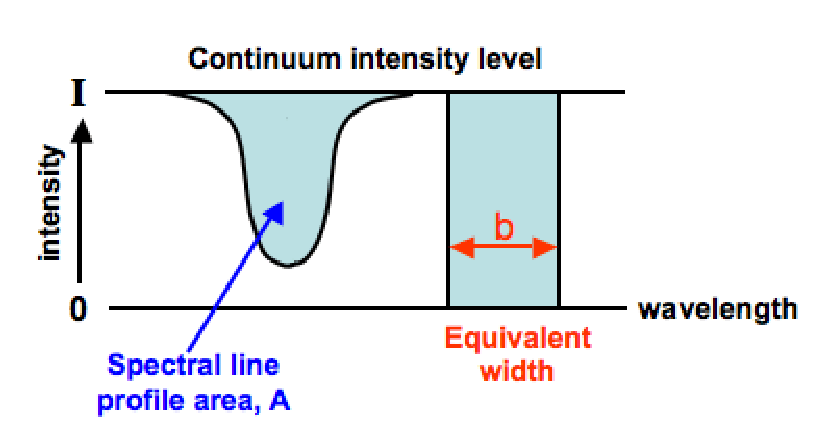
\includegraphics[height=5 cm]{pics/equivalent_width}
\caption{a) Illustration of a spectral line and its equivalent width. From: ()}
\label{ew}
\end{figure}

The EW is thus measured in wavelength units (\AA{}  or m\AA). Mathematically we have

\begin{equation}
 W=\int_{-\infty}^{\infty} \frac{I_c-I_\lambda}{I_c}d\lambda,
\end{equation}
where $I_c$ is the intensity of the continuum and $I_\lambda$ is the intensity of the wavelength at each $d\lambda$.

From the accurate measurement of the EW of weak lines we can get the abundances of species and also calculate some stellar parameters (temperature, surface gravity).

\subsection{The Abundance Dependence}
\label{abdep}

As the abundance increases, line strength also increases, as expected. However, the EW does not change linearly with abundance, as we can see in Fig. (\ref{cog}a). 
\begin{figure}[h]
\centering
\subfigure[]{
\includegraphics[height=5 cm]{pics/branco}}
\subfigure[]{
\includegraphics[height=5 cm]{pics/branco}}
\caption[EW and Profile dependence of abundance] {a) Typical curve of growth in a model photosphere ; b) Line profile change with chemical abundance of the absorption species. The dots in (a) correspond to the dots in (b).}
\label{cog}
\end{figure}

There are three different phases. The first one corresponds to the weaker line behaviour, where the Doppler core dominates (?) and the EW is proportional to the abundance $A$. The second phase begins when the central depth aproaches the maximum value and the line saturates and grows assymptoticaly towards a constant value. The third one starts as the optical depth of the line wings becomes significant compared to the absorption of the continuum. We are only interested in the first phase, where the behaviour of the curve is linear.

Every spectral line shows a similar behaviour. A figure like Fig. (\ref{cog}a) is called a curve of growth. Fig. (\ref{cog}b) shows the line profile change with chemical abundance of the absorbing species.

\subsection{The Temperature Dependence}

Temperature is the most important variable in determining the line strength.  This can be easily seen in the excitation and ionization process equations (section \ref{LTE}).
We can appreciate the behaviour of the EW of a typical weak line with $T_{eff}$ depicted by Fig. (\ref{ewdep}a). Four cases are of interest:
\begin{enumerate}
 \item weak line of a neutral species with the element mostly neutral.
 \item weak line of a neutral species with the element mostly ionized.
 \item weak line of an ion with the element mostly neutral.
 \item weak line of an ion with the element mostly ionized.
\end{enumerate}
\begin{figure}[h]
\centering
\subfigure[]{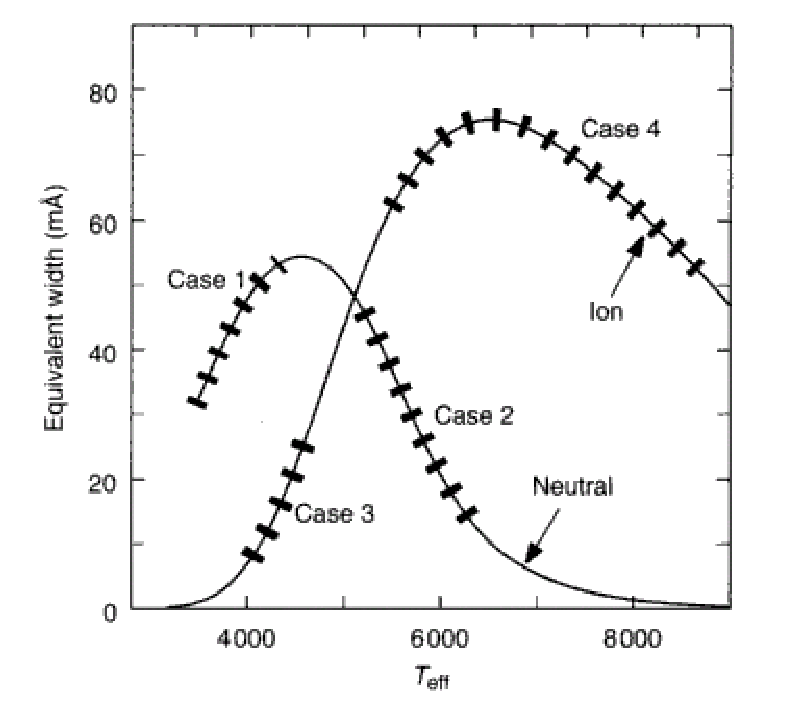
\includegraphics[height=4 cm]{pics/ewtemptempeps}}
\subfigure[]{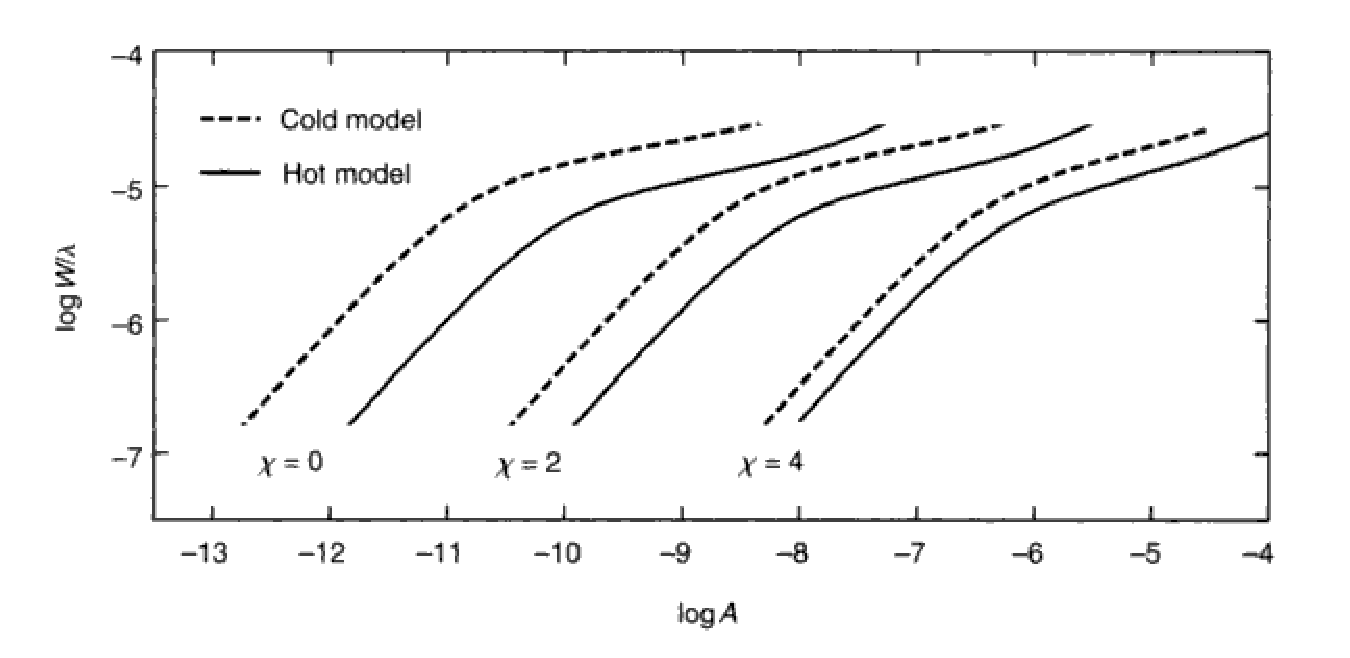
\includegraphics[height=4 cm]{pics/cogtempeps}}
\caption[EW dependence on Temperature and Pressure] {a) Plot of the behaviour of the EW of typical weak metal lines with $T_{eff}$. The cases discussed in the text are shown.; b) Curves of growth corresponding to different temperatures, for three excitation potentials.} %Profiles of FeII $\lambda4508$ shown for several values of surface gravity ($gcm/s^2$). Inset: change in EW.}
\label{ewdep}
\end{figure}

In most situations, an increase in $T_{eff}$ implies an increase in excitation (cases 1,3 and 4). Most lines have a maximum in strength. The decrease can be accounted for from the increase in continuous absorption, which comes from an increase of electron pressure with $T_{eff}$ (case 4)  or from the ionization of the absorbing species (case 2). Note that the weakening of the line due to an increase of continuous absorption also affects the lines in case 1 and 3. However, this effect is weak compared to the excitation one. 

The direction and strength of change will depend on the Teff and on the excitation potential of the line. For stars similar to the Sun, cases 2 and 4 apply because most elements are ionized. Solar lines of neutral species almost always decrease in strength with $T_{eff}$, but ionized species have the opposite behaviour. 

Temperature differences can shift a typical curve of growth, as we can see in Fig. (\ref{ewdep}b).

\subsection{The pressure dependence}

The pressure effects are visible in different ways. The dominant effect in weak lines is the change in the ratio of line absobers to the continuum absorption (ionization equilibrium). To account for pressure effects we must consider gas pressure ($P_g$) and electron pressure ($P_e$). In cool stars, the pressure can be approximated by $P_g\approx C g^{2/3}$ and $P_e\approx C' g^{1/3}$, where $C$ and $C'$ are constants and $g$ is the star's surface gravity. In this case, pressure can be translated into approximate gravity dependences for the F,G and K stars, which is our case. %We can see such dependence illustrated in Fig. (\ref{ewdep}b) 

It's important to emphasize that pressure effects in stellar spectra are much weaker that temperature effects. For weak metal lines in cool stars, we can enumerate the following rules, based on Eq. (\ref{Saha}):

\begin{enumerate}
 \item weak lines formed when most of the element is in the next higher ionization stage are insensitive to pressure changes.
\item weak lines formed where most of the element is in that same ionization stage are pressure sensitive: lower pressure cause greater line strength.
\item weak lines formed where most of the element is in the next lower ionization stage are very pressure sensitive. Lower pressure enhances the lines.
\end{enumerate}

Regarding solar type stars, cases 1 and 2 are more common (neutral and first ion species, respectively).

Surface gravity can change the percieved abundances of a certain element. We can see in Fig. (\ref{cogpmt}a) the change of the curve of growth of an ion (Fe II) with the surface gravity.

\begin{figure}[h]
\centering
\subfigure[]{
\includegraphics[height=5 cm]{pics/branco}}
\subfigure[]{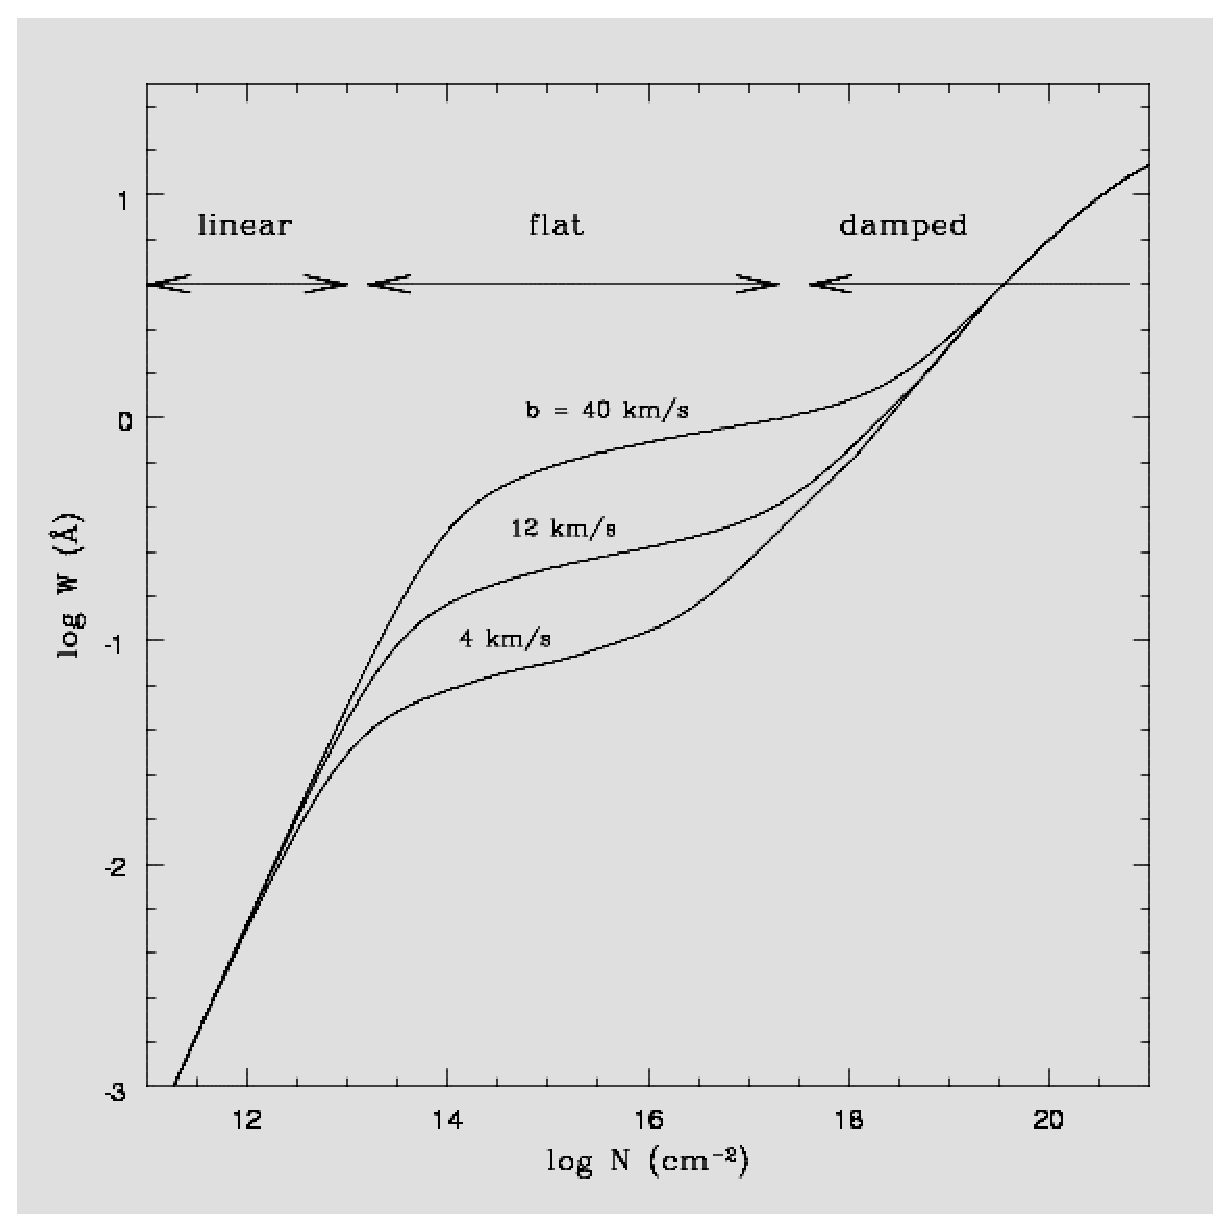
\includegraphics[height=5 cm]{pics/cogmt}}
\caption[Curves of growth dependent of surface gravity and microturbulence] {a) Curves of growth dependent of surface gravity. It only affects ions; b) Curves of growth with different values of microturbulence.} %Profiles of FeII $\lambda4508$ shown for several values of surface gravity ($gcm/s^2$). Inset: change in EW.}
\label{cogpmt}
\end{figure}

If log(g) is known then the neutral and ion lines should give the same abundance. If log(g) is unknown, it can be determined by forcing the ion and neutral solutions to give the same abundance (spectroscopic surface gravity)(\textcolor{red}{confirmar isto}).

\subsection{Microturbulence}

%As we have seen, the slope in the curve of growth is much less in the saturation part of the curve of growth. This means that any error in the measurement of the EW in this area will translate into a much greater error in the final abundance. One more reason to use the linear portion of the curve of growth. 

Microturbulence is almost always incorporated into abundance analysis because it explains that the EW of saturated lines are greater than predicted. The Fig. (\ref{cogpmt}) shows how microturbulence delays the saturation. 

%To determine $\xi$ we fit the EWs of the weakest lines and then we adopt the theoretical curve that has the best fit of the data in the saturation portion.

Deviations from LTE can also cause similar changes in the curve of growth. This effect is much more important in strong lines \textcolor{red}{(entao pk raio e q se aplica na nossa analise????)}. The chemical abundances deduced from weak lines are not influenced by these mechanisms.
\textcolor{red}{mas nesse caso porque usamos o microturbulencia se usamos apenas a parte linear da curva? Porque isto entra no MOOG se n e usado?}


\section{scaling} 

\textcolor{red}{meter ou nao eis a questao. O MOOG faz scaling? Bem, de qq forma ja esta incorporado na seccao anterior agora...ptt penso q e para tirar}

%\subsection{Temperature effects}

%If a careful analysis is performed the errors derived from temperature should not exceed 100K and might be smaller than that. 
%Temperature enters through the ionization equilibrium and shifts the curve of growth as we can see in Fig. (\ref{}).
%A simple way to test this effects is to repeat the calculation changing only the temperature and see the output of the abundance. This should not be a serious problem if the determination of the temperature is acceptable. 


\section{Derivation of Abundances} 
\textcolor{red}{preciso de clarificar esta seccao antes de a passar para cima}

``As outlined the direct computational approach can be used, where all the scaling rules are ignored and the abundances are derived from a model atmosphere calculation of a curve of growth for each line'' (\textcolor{red}{afinal usamos as scaling rules, a direct computational approach ou ambas? - preciso de tirar esta duvida asap})
The abundances are derived from a model atmosphere calculation of a curve of growth for each line. If all parameters are correct, all the abundances of all spectral lines of a certain element will be the same. Therefore, the abundance should be independent of the stellar parameters and of the EW. If it's not, there must be an error in some value of the stellar parameters, in the measured EWs or even in the model itself, if NLTE effects became important. Errors can grow a lot if we have few lines to measure the EW, where line blending is severe or where atomic constants are not well known.

\section {Differential analysis}
\label {difanal}

%By means of differential analysis or, in other words, comparing one star (normally the Sun) with another (in this case a star similar to the Sun) the oscillator strengths cancel out and the ratio of the abundances in the stars is known. This can only be applied to stars with similar stellar parameters, especially effective temperature and surface gravity. If there are errors involved in the calculations, they are the same for both stars and by the same amount.


Differential analysis consists in comparing abundances between stars. This is a good method to study similar stars, which is our case.  The comparison is made between a reference star (normally the Sun) and a star of unknown composition, deriving the value $A/A_{ref}$ for the elements of interest, where $A_{ref}$ is the abundance of the reference star. The atomic parameters for each line are the same for both stars. Only the EW changes. The output abundance will be the logarithm of the abundance of the star to the solar abundance and will be denoted as, e.g. $[X/H]$, where $[X/H]=log[A(X)_{star}/A_\oplus(X)]$. Differential analysis based on weak lines assumes that the ionization fraction is the same in both stars %(e...). 
The advantage of differential analysis is that one obtains an empirical fix on the oscilator strength value. 

We need to note that deviations from LTE typically cause errors of no more than a few per cent. We also need to note that this abundance is only valid in the atmosphere of the star. The abundance of its interior might be totally different.

The solar composition is the standard composition against the other stars are compared and therefore is used as standard for many differential stellar analysis and for the basic chemical mix entering many stellar photosphere models. The mass fraction used is typically X=0.735 for hidrogen, Y=0.248 for helium and Z=0.017 for all other elements. The solar system composition is established from measurments of the Earth, planetary atmospheres and especially from meteorites. We can use e.g. \citet{Anders-1989} to obtain the solar abundances. 

%\section {The synthesis method}

%The computation of a complete spectral interval where all the observed lines are included is called a synthesis. This method is especially useful when line blending is severe (cool stars) or stars showing large rotational broadening. It works best when all spectral lines can be identified and all its parameters are known and consists in the arbitrary adjustment of abundances, oscilator strenghts and line and doppler broadening until the spectrum is reproduced. (Sneden 1973). 

\section{Galactic Variations}
\textcolor{red}{mmmm....valera a pena por ou deixa-se para o paper...so se meter depois de dia 25, o q dizem?}

%%%%%%%%%%%%%%%%%%%%%%%%%%%%%
%Capítulo 3 %%%%%%%%%%%%%%%%%
%%%%%%%%%%%%%%%%%%%%%%%%%%%%%

\chapter {Determination of the abundances of refractory elements \textcolor{red}{mudar titulo?}}

The details of the technique used for the determination of the abundances will be explained in the following chapter.  It's important to emphasize that this an homogeneous study. It means that the spectra used to measure the EW of the atomic lines were taken with the same instrument (HARPS) and reduced and normalized with the same methodology; and that the calculated atomic and stellar parameters were based on the same atmospheric models.

\section {Spectral Data}

The HARPS 'high precision' GTO subsample was obtained with the HARPS spectrograph at the ESO La Silla 3.6m telescope. It is composed of 451 stars selected from the volume limited stellar sample of the solar neighborhood (< 20 pc), studied with the CORALIE spectrograph \citep{Udry-2000} and from a group of planet host stars of the southern hemisfere. The total number of planet-bearing stars  is 66. Every star in the catalogue is slowly rotating, non evolved and with low chromospheric activity. 

The GTO program main goal is the detection of very low mass exoplanets aiming to push the RV accuracy below $1m/s$ \citep{Mayor-2003b}. We will use the combined spectra of a considerable quantity of high resolution high S/N spectral samples to calculate the abundances of several species. 

The individual spectrum were reduced using the HARPS pipeline and later combined using IRAF after correcting for its radial velocity. The final spectra have a resolution of $R\sim110.000$ and a signal to noise ratio ranging from $\sim70$ to $\sim2000$ depending on the amount and quality of the original spectra. Nine tenths of the spectra have S/N higher than 200.  

In order to average out stellar oscillations, the observations lasted at least 15 minutes. Sometimes it's necessary to separate the observations in several exposures in order to avoid the saturation of the detector. The result is a very high quality spectrum of each star. 

The solar spectrum was collected from the solar light reflected by Ceres. It was also obtained with the HARPS spectrograph. This spectrum has the same resolution of the star's spectra and a S/N ratio of $\sim250$. 

A sample of the 'high precision' GTO catalogue is shown in Table (\ref{cat_sample}). The stellar parameters of this table were determined by Sousa (2008). The full catalogue is available at $http://www.astro.up.pt/\sim sousasag/harps\_gto\_catalogue.html$. 

\begin{table}[h]
  \centering
\caption[Sample table of the HARPS GTO ``high precision'' spectroscopic catalogue.]{Sample table of the HARPS GTO 'high precision' spectroscopic catalogue. Each line gives the star's name, effective temperature ($T_{eff}$),spectroscopic surface gravity ($log\,g_{spec}$), microturbulence ($\xi_t$), mettalicity ([Fe/H]), signal to noise ratio of the spectrum (S/N) and if the star hosts planets. All parameters were obtained by Sousa 2008.}
  \label{cat_sample}
  \begin{tabular}{ c r@{$\pm$}l r@{$\pm$}l r@{$\pm$}l r@{$\pm$}l c c}
  \hline
  \hline
Star ID & \multicolumn {2}{c}{$T_{eff}$} & \multicolumn {2}{c}{$log\,g_{spec}$} & \multicolumn {2}{c}{$\xi_t$} & \multicolumn {2}{c}{[Fe/H]} & S/N & planet host? \\ 
& \multicolumn {2}{c}{[K]} & \multicolumn {2}{c}{[$cm\,s^{-2}$]} & \multicolumn {2}{c}{[$km\,s^{-1}$]} & \multicolumn {2}{c}{ } &  &  \\
\hline
... & \multicolumn {2}{c}{...} & \multicolumn {2}{c}{...} & \multicolumn {2}{c}{...} & \multicolumn {2}{c}{...} & ... & ... \\
HD117207 & 5667 & 21 & 4.32 & 0.04 & 1.01 & 0.02 & 0.22 & 0.02 & 252.60 & yes \\
HD117618 & 5990 & 13 & 4.41 & 0.02 & 1.13 & 0.01 & 0.03 & 0.01 & 613.22 & yes \\
HD119638 & 6069 & 16 & 4.42 & 0.03 & 1.22 & 0.02 & -0.15 & 0.01 & 1163.50 & no \\
HD119782 & 5160 & 34 & 4.44 & 0.06 & 0.79 & 0.07 & -0.07 & 0.02 & 479.70 & no \\
HD121504 & 6022 & 11 & 4.49 & 0.03 & 1.12 & 0.01 & 0.14 & 0.01 & 526.01 & yes \\
HD122862 & 5982 & 13 & 4.23 & 0.02 & 1.29 & 0.01 & -0.12 & 0.01 & 1338.76 & no \\
HD123265 & 5338 & 44 & 4.29 & 0.07 & 0.85 & 0.08 & 0.19 & 0.03 & 354.26 & no \\
HD124106 & 5106 & 39 & 4.49 & 0.08 & 0.80 & 0.09 & -0.17 & 0.03 & 361.54 & no \\
HD124292 & 5443 & 22 & 4.37 & 0.04 & 0.77 & 0.03 & -0.13 & 0.02 & 975.63 & no \\
HD124364 & 5584 & 14 & 4.48 & 0.02 & 0.83 & 0.02 & -0.27 & 0.01 & 451.62 & no \\
... & \multicolumn {2}{c}{...} & \multicolumn {2}{c}{...} & \multicolumn {2}{c}{...} & \multicolumn {2}{c}{...} & ... & ... \\
\hline
\end{tabular}
\end{table}





\section {The HARPS Spectrograph}

Originally designed to detect low mass exoplanets by RV up to the  1m/s threshhold, HARPS can also be used to acquire high resolution high S/N spectra of planet host stars. This spectra can then be used for abundance studies, which is our case. 

HARPS is a fiber-fed, cross dispersed echelle spectrograph. It operates at a constant 17$^o$C, with a pressure < 10$^{-2}mbar$. It is located in the Coude' floor of the ESO La Silla 3.6m telescope. Two fibers, an object and a reference fibre fed the spectrograph with light from the telescope and from the calibration lamps. The light is reimaged by the internal optics onto a mosaic of two 2k4 CCDs where two spectra of 72 orders are formed. The spectral region goes from 380 to 690nm. At the resolution of 115.000, each spectral element is sampled by 3.2 CCD pixels. For further details refer to \citet{Mayor-2003b}. 

\textcolor{red}{chega ou mete-se mais alguma coisa? fontes de ruido?}



%The most obvious error source is photon noise: it is the one coming from the finite number of photons collected in a stellar spectrum. The fundamental uncertainty on the RV depends both on the number of recorded photons and on the intrinsic slope of the spectrum. 
%Stellar Oscillation Noise. Solar type stars show p mode oscillations with periods of a few minutes and amplitudes of a few m/s. However some of these signals can superimpose. The present strategy regarding this noise is to integrate over a few characteristic periods to average out these effects as much as possible. This maintains this noise below 1 m/s.
%Stellar activity related jitter. Magnetic phenomena at the surface of solar type stars can induce RV perturbations in the order of 100 m/s. This prevents completely the use of RV technique to detect planetary companions. Stars in the HARPS catalogue are chosen for showing low chromospheric activity and slow rotation. to ensure that these effects stay below a few m/s. 


\section {Identification and selection of the Spectral Lines}

The first part of this work consisted in the identification and selection of the weak spectral lines of the following species: alpha group elements (Si, Ca, Ti, Sc), iron peak elements (Mn, V, Cr, Co, Ni) and also Na, Mg and Al. The absorption lines of some of the first ionized species (Ti II, Sc II, Cr II)  were also studied.

\textcolor{red}{falta meter aqui qualquer coisa sobre a origem dos elementos nao?}

\subsection {Using VALD to obtain the initial list of spectral lines}
\label{VALD}
Our study started with the request at the Vienna Atomic Line Database (VALD - Kupka 1999, Ryabchikova 1999)  of all spectral lines and their atomic parameters (wavelength, oscillator strength,excitation potential) %created with a synthetic spectra (Kurucz 1993 - \textcolor{red}{confirmar!}) 
from $4500$ to $6910$ \AA. The request was done via the internet ($http://www.astro.uu.se/\sim vald/$). These lines were obtained from a synthetic spectra based on Kurucz Atlas 9 plane-parallel model atmospheres (Kurucz 1993).

Inside VALD, the 'extract stellar' option was chosen and the following parameters were inserted: Spectral Region: $4500-6910$ \AA ; $T_eff=5777\, K$; $log g=4.44\,dex$; $\xi_t=1.0\,kms^{-1}$; $detection limit=0.05$, where $T_eff$ is the effective temperature, $log\,g$ is the surface gravity and $\xi_t$ is the microturbulence of the star. The detection limit was set to 0.05. This means that only the spectral lines with central depths greater than 5\% of the continuum were accepted. The stellar and atomic parameters inserted in the model are those of the Sun. The goal was to use the most approximate model of the Sun as possible in order to obtain the correct spectral lines.

The acquired output contained the wavelength, excitation potential, estimated line depth and oscillator strength for each spectral line. The 'extract stellar' option has the advantage of supplying all the spectral lines. Sometimes, our spectral line is not there. However, there might be a perfectly good line in its place (or a line slightly blended with ours) with almost the same wavelength but from other element. When this happens, we have to reject the line. This helped a lot in a first identification and selection of the 'good' lines. 

\subsection {Using IRAF to identify the 'good' lines}

With the IRAF (http://iraf.noao.edu/) splot tool, we opened a noiseless synthetic spectrum of the Sun (Kurucz Solar Flux Atlas - \citet{Kurucz-1984} ) with a resolution $R\sim100.000$ and we carefully checked for the existence of the lines of interest.

We only chose isolated or lightly blended lines. Then, we measured their EW. All lines with EWs lower than 5 m\AA\, or inside the wings of strong lines (e.g. $H_\alpha$, $H_\beta$, strong Ca I and Mg I lines) were excluded. A classification system was made, ranging from 1 (blended, distorted or hard to read lines) to 5 (totally isolated lines). 364 lines were selected in this first phase, from an initial list of 2169 lines. 

It's worth noting two things regarding the manual measurement of spectral lines using IRAF: we should always choose a region of at least 1 \AA{} to each side from the center of the line of interest and deconvolute all lines in that region (1); we should never measure a line above the continuum: when choosing the points that will determine the region of interest, it is wise to target slightly below the highest points of the continuum (2).

\subsection {Measuring the EW of the lines with ARES}
\label{ARES}
We used ARES (Automatic Routine for Line Equivalent Widths - \citep{Sousa-2007}) to automatically measure the equivalent widths of our lines. First, we analyzed the lines of two different spectra: one is a resolution and noise degraded spectrum of the Kurucz Solar Flux Atlas ($R=110.000$, $S/N\sim350$) and the other is a spectrum taken with the HARPS spectrograph using the Ceres asteroid, (Collection of HARPS solar spectra: http://www.ls.eso.org/lasilla/sciops/3p6/harps/monitoring/sun.html) with $R\sim110.000$ and $S/N\sim250$ \textcolor{red}{confirmar valores de R e S/N}.

The measurement of the EWs was done one line at a time and was monitored with a graphical interface (plots\_flag=1 within the 'mine.opt' file). This way we could see if the lines were being fitted properly. 

The EW measurement in these very similar spectra allowed us to establish a tighter criteria: if we obtained an absolute value of the ratio between EWs (measured in both spectra) for the same line greater than 0.10, we  discarded this line. Then, every line with a difference of EWs,measured in both spectra, greater than 1 m\AA{} was investigated to see if it was subjected to blending effects and discarded if appropriate. These criteria are important because the abundance is very sensitive to variations in the EW. Therefore, if we are going to use a model atmosphere for each star to predict the abundances, we will need a line list with the real EWs as close as possible to the ones measured with the synthetic spectrum based on the same atmosphere model. (\textcolor{red}{se nao e por isto entao porque e??? discutir!}

In order to optimize the calculation of the EWs, we chose the following ARES parameters (within the 'mine.opt' file): smoother=4; space=2, lineresol=0.07, miniline=5 and rejt=0.996, where 'smoother' is a parameter to adjust the noise smoothing (1 to 4, the bigger the number, the greater the smoothing produced in the spectrum), 'space' is the interval, in angstrom, used for the computation of each line; 'lineresol' sets the line resolution (in \AA) of the input spectra (if the program finds two lines closer than this value he will treat them as one line),  'miniline' is the minimum value of line strength (in m\AA{}) accepted to write a line in the output file and 'rejt' is a parameter for the calibration of the normalized continuum (0 to 1). The 'rejt' is the most important parameter for the correct automatic determination of the continuum (\citeauthor{Sousa-2006} \citeyear{Sousa-2006}, \citeyear{Sousa-2007}). The higher the S/N ratio the higher the rejt parameter should be (refer to table (\ref{}).

We also repeated the classification process for both spectra. All lines with classification 1 were rejected and lines with 2 were investigated and discarded when appropriate. Aditionally, all lines situated in regions of strong variation of the continuum as well as lines with bad fits were excluded. At the end of the process, we had a new list with 284 lines. 

\subsection {Calculating new oscillator strengths}
\label{newloggf}
The EWs of the new list of lines and a Kurucz grid model for the Sun \citep{Kurucz-1993} having ($Teff=5777$, $log\, g=4.44$, $[Fe/H]=0.0$ and $\xi_t=1.0$) were used to calculate new semi-empirical atomic oscillator strengths for the spectral lines from an inverted solar analysis. This was necessary because \textcolor{red}{(...)}

The calculations were carried out with the 'ewfind' driver of the 2002 version of the LTE stellar line analysis program MOOG \citep{Sneden-1973}. The fixed solar abundances used in MOOG were taken from Anders and Grevesse (1989) except (...). The excitation potential and the initial value of $log(gf)$ of every line came from the VALD database, as referred in subsection (\ref{VALD}). \textcolor{red}{Sera relevante meter aqui os parametros do ewfind.par? Parece-me demasiado tecnico. e necessario dizer porque e q se calcula novos valores}


%The parameters used with ewfind that are relevant to emphasize are the following: molecules=1 (it calculated the molecular equilibrium), flux/int=0(perform integrated flux calculations) and damping=2 (use the Un . All other parameters were taken by default. For further information refer to MOOG Manual (...).
The objective was to 
Our goal here is to calculate a 

The calculation of the new $log(gf)$ values was done with an iterative FORTRAN program. For each individual line, we input at MOOG the fixed atomic parameters, the fixed solar EWs and a variable value of the oscillator strength (starting with the $log(gf)$ provided by VALD). At the end of the iteration, we got a certain value of the abundance as output. The true value of $log(gf)$ is obtained when the value of the abundance for each element equals its solar abundance. The iteration ends when the correlation coefficients between the abundance and $\chi_l$ and between the abundance and the reduced equivalent width (RW) are zero. In order to achieve the convergence of abundances, we used a simple bisection method in the iteration. It takes no more than a few minutes to obtain the correct log(gf) for all lines. 

If we invert this analysis, we can use the new oscillator strengths to obtain the abundance of any element for every star. \textcolor{red}{preciso perceber isto melhor. discutir com o Nuno...mas este e mesmo o verdadeiro valor de log(gf) ou e so um artificio para fixar os parametros e calcular a abundancia por analise diferencial???}.

\subsection {A test using the Sun Abundance values}

In order to confirm that the calculated $log(gf)$ values were correct, we made a test using the measured EWs of Sun's Ceres spectrum and a \citet{Kurucz-1993} atmospheres model (with the Sun's parameters) to calculate the abundances using MOOG 'abfind' driver . This time, we did the inverse analysis: the $log(gf)$ and the EW values were fixed and the abundance was calculated by converging to a value that matches the conditions described in subsection (\ref{newloggf}). The average values of the abundances are within 0.01 of the expected value except for Al ($\Delta Ab= 0.03$ with two lines), Sc I ($\Delta Ab=0.03$ with three lines) and V ($\Delta Ab=0.02$ with 14 lines). We shall watch these elements for biases. No further lines were removed at this point. \textcolor{red}{por aqui uma tabela com estes dados?}

\subsection {The molecular equilibrium}

Some of the analysed species may form molecules. This tendency increases for lower temperatures and can change the abundance of the element in question, if not properly corrected. Obviously, this effect is stronger in cooler stars.

In order to find if the use of molecular equilibrium was needed to correct the abundance of certain species, we measured the EWs using ARES and calculated the abundances for the coolest star in our sample, HD218511, using the MOOG code ('abfind' driver) and a Kurucz model atmosphere with the star's parameters ($T_{eff}=4556\,K, log\,g=4.31, vtur=0.41, [Fe/H]=-0.10$).  This calculation was done with two different values of the 'abfind' driver parameter 'molecules'. If 'molecules' was set to zero, MOOG did not use molecular equilibrium. If molecules was set to '1', MOOG would calculate the abundance with the molecular equilibrium correction. No change in the abundance of any element was found. Therefore, we chose not to use molecular equilibrium when calculating the abundances.

\subsection {Testing a small sub sample containing 20 stars} 
\label{20stars}
In order to finish the selection of the spectral lines, two different groups of stars were chosen. The first group contained the 10 stars with $T_{eff}$ closer to $5000 K$, hereafter 'cool group'. The second group contained the 10 stars with $T_{eff}$ closer to the Sun's temperature ($5777 K$), hereafter 'hot group'. We will calculate the abundance of both groups separately and then we will observe the dispersion and difference to the mean value of abundance of each line, for every element and make the selection of the lines based on an appropriate criteria. \textcolor{red}{meter aqui uma tabela deste sub sample?}

This analysis is very important. With it, we can find lines that yield wrong abundance values due to an incorrect measurement of the EW (originated in blending effects (stronger in cooler stars) or in a poor position in the continuum), due to errors of the analysis methodology (the differential analysis used is based on the Sun and the further away a star is from the Sun's parameters the greater the errors the analysis will yield: this is especially true for temperature differences), or simply due to systematic errors of unknown origin.

First, we measured the EWs with ARES. The program parameters were the same ones used in subsection (\ref{ARES}) except 'rejt' that changed with the S/N ratio of each star, according to Table \ref{} (Sousa 2008). 

Then, we made a small FORTRAN program that used the 'abfind' driver within MOOG and a grid of Kurucz (1993) Atlas9 atmospheres to calculate the abundance of the individual elements. We can see in Fig. (\ref{Ni20}) the difference between the abundance of each line and the mean abundance of the respective star, for Ni, shown as example. The red and the blue dots correspond to the 'hot' and 'cool' groups respectively. This difference will be referred as $\Delta Ab$. The cyan and black stars are the mean value of $\Delta Ab$ of the hot and the cool group, respectively, and the error bars represent the standard deviation of these mean values. 

\begin{figure}[h]
\centering
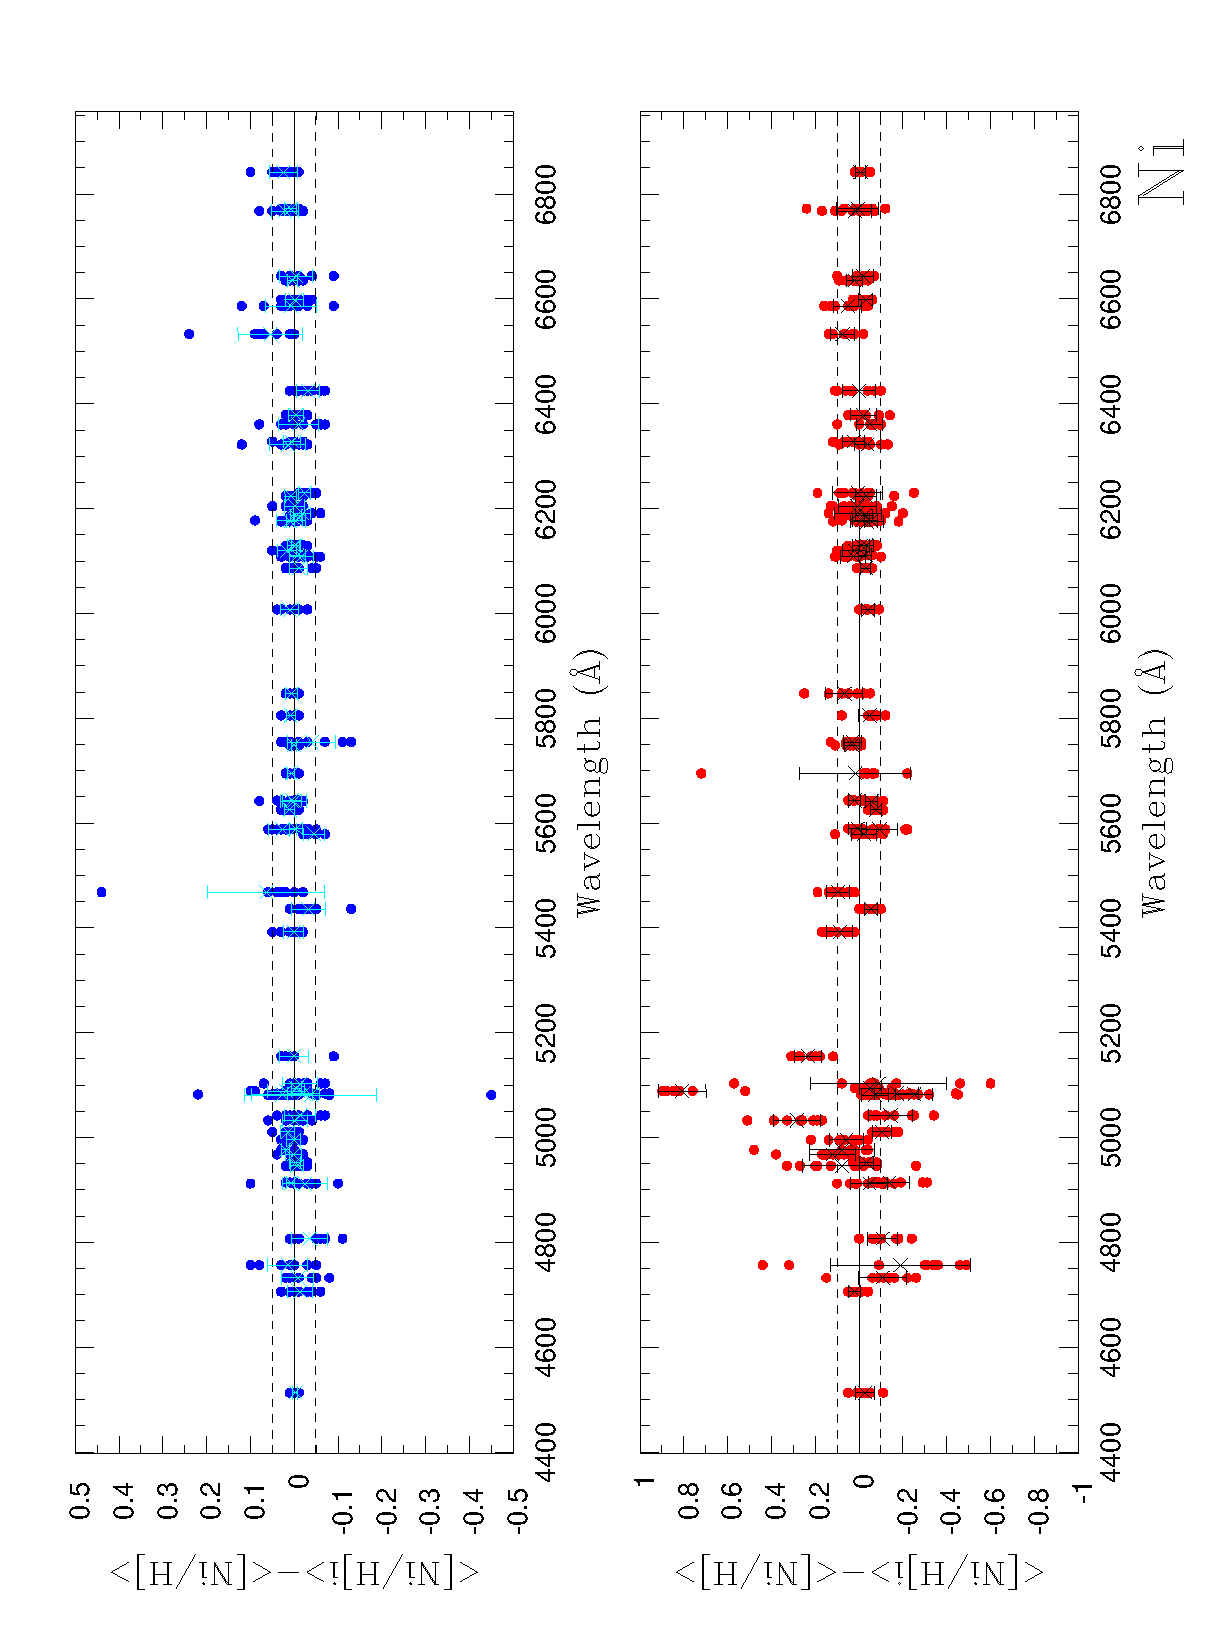
\includegraphics[width=10 cm]{pics/Ni20.eps}
\caption[20 star delta ab graphics]{Selection of the stable lines for Ni based on an analysis of 20 stars. (...)}
\label{Ni20}
\end{figure}

Following the analysis of Fig. ({\ref{Ni20}), the lines were selected according to two different criteria: all lines within the hot group with $\Delta Ab$ or/and with a dispersion greater than 0.05 dex were excluded (1); all lines of the cool group with $\Delta Ab$ or/and  with a dispersion greater than 0.1 dex were excluded (2). It was taken great care in identifying stray points clearly out of the $2\sigma$ distribution (due to bad pixels, cosmic rays or other unknown effects) that could alter the true value of the mean or the dispersion of a certain line. This is the case, for example, of the 5468.11 \AA{} line in the hot group or the 5694.99 \AA{} line in the cold group that could have been excluded if the criteria was strictly obeyed. 

After the selection of the spectral lines according to this criteria, we created a final list of lines as shown in Table (\ref{loggf}). 

\begin{table}[h]\scriptsize
\label {loggf}
  \centering
\caption[Atomic parameters of the spectral lines]{Atomic parameters and measured solar equivalent withs of the spectral lines used to determine the abundance of the elements} 
  \begin{tabular}{c c c c | c c c c | c c c c}
\hline
\hline 
$\lambda$(\AA) & $\chi_l$ & $log\,gf$ & $EW\,(m$\AA{}) &$\lambda\,\ $(\AA{}) & $\chi_l$ & $log\,gf$ & $EW\,(m$\AA{}) &$\lambda\,\ $\AA{} & $\chi_l$ & $log\,gf$ & $EW\,(m$\AA{}) \\
\hline
\textbf{Na I} &  & &  & 5662.16 & 2.32 & -0.123 &  23.5 & 5301.05 & 1.71 & -1.950 &  19.5 \\
6154.23 & 2.10 & -1.622 &  36.6 & 5716.46 & 2.30 & -0.869 &   5.7 & 5342.71 & 4.02 &  0.606 &  32.3 \\
6160.75 & 2.10 & -1.363 &  54.3 & 5739.48 & 2.25 & -0.781 &   7.7 & 5352.05 & 3.58 &  0.004 &  24.4 \\
\textbf{Mg I} &  & &  & 5766.33 & 3.29 &  0.326 &   9.6 & 5647.24 & 2.28 & -1.594 &  14.0 \\
5711.09 & 4.35 & -1.777 & 105.6 & 5965.84 & 1.88 & -0.492 &  26.7 & 6814.95 & 1.96 & -1.822 &  18.8 \\
6318.71 & 5.11 & -2.046 &  39.1 & 5978.55 & 1.87 & -0.602 &  22.6 & \textbf{Ni I} & & &  \\
6319.24 & 5.11 & -2.300 &  25.2 & 6064.63 & 1.05 & -1.941 &   8.3 & 4512.99 & 3.71 & -1.467 &  19.4 \\
\textbf{Al I } &  & &  & 6126.22 & 1.07 & -1.416 &  22.1 & 4705.92 & 3.66 & -1.881 &   9.8 \\
6696.03 & 3.14 & -1.571 &  36.2 & 6258.11 & 1.44 & -0.435 &  51.5 & 4732.46 & 4.11 & -0.583 &  42.8 \\
6698.67 & 3.14 & -1.886 &  21.1 & 6261.10 & 1.43 & -0.491 &  49.2 & 4806.99 & 3.68 & -0.593 &  61.6 \\
\textbf{Si I} &  & & & 6599.12 & 0.90 & -2.069 &   9.3 & 4912.03 & 3.77 & -0.712 &  51.8 \\
4947.61 & 5.08 & -2.307 &  18.3 & \textbf{Ti II} & & & &  4946.04 & 3.80 & -1.224 &  26.2 \\
5517.54 & 5.08 & -2.496 &  12.9 & 4583.41 & 1.16 & -2.840 &  31.8 & 4952.29 & 3.61 & -1.261 &  32.3 \\
5645.61 & 4.93 & -2.068 &  35.8 & 4636.33 & 1.16 & -3.152 &  19.8 & 4976.33 & 1.68 & -3.002 &  37.7 \\
5684.49 & 4.95 & -1.642 &  61.2 & 4657.20 & 1.24 & -2.379 &  49.3 & 4995.66 & 3.63 & -1.611 &  17.9 \\
5701.11 & 4.93 & -2.034 &  37.7 & 4708.67 & 1.24 & -2.392 &  48.9 & 5010.94 & 3.63 & -0.901 &  48.8 \\
6125.02 & 5.61 & -1.555 &  31.7 & 4911.20 & 3.12 & -0.537 &  52.3 & 5081.11 & 3.85 &  0.064 &  93.5 \\
6145.02 & 5.62 & -1.425 &  38.8 & 5211.54 & 2.59 & -1.490 &  32.8 & 5094.41 & 3.83 & -1.108 &  30.3 \\
6195.46 & 5.87 & -1.666 &  17.1 & 5490.70 & 1.57 & -2.800 &  20.0 & 5392.33 & 4.15 & -1.354 &  12.0 \\
6237.33 & 5.61 & -1.116 &  61.1 & \textbf{V I}  & & & & 5435.86 & 1.99 & -2.432 &  51.7 \\
6243.82 & 5.62 & -1.331 &  44.8 & 5670.85 & 1.08 & -0.482 &  18.8 & 5468.11 & 3.85 & -1.641 &  12.0 \\
6721.85 & 5.86 & -1.156 &  44.0 & 5727.05 & 1.08 & -0.015 &  38.8 & 5578.73 & 1.68 & -2.649 &  56.4 \\
6741.63 & 5.98 & -1.625 &  15.5 & 6039.73 & 1.06 & -0.747 &  12.4 & 5587.87 & 1.93 & -2.479 &  52.9 \\
6800.60 & 5.96 & -1.787 &  11.5 & 6081.45 & 1.05 & -0.692 &  14.1 & 5589.36 & 3.90 & -1.148 &  26.7 \\
\textbf{Ca I} & & &  & 6090.21 & 1.08 & -0.150 &  33.5 & 5625.32 & 4.09 & -0.731 &  37.8 \\
5261.71 & 2.52 & -0.677 &  97.7 & 6119.53 & 1.06 & -0.451 &  21.6 & 5641.88 & 4.11 & -1.017 &  24.1 \\
5349.47 & 2.71 & -0.581 &  94.6 & 6243.11 & 0.30 & -1.067 &  27.8 & 5643.08 & 4.16 & -1.234 &  15.1 \\
5512.98 & 2.93 & -0.559 &  84.8 & 6251.83 & 0.29 & -1.431 &  15.0 & 5694.99 & 4.09 & -0.629 &  43.1 \\
5867.56 & 2.93 & -1.592 &  25.1 & \textbf{Cr I} & & &  & 5748.36 & 1.68 & -3.279 &  28.0 \\
6156.02 & 2.52 & -2.497 &   9.6 & 4575.11 & 3.37 & -1.004 &  10.0 & 5754.66 & 1.93 & -2.014 &  75.0 \\
6161.29 & 2.52 & -1.313 &  60.6 & 4626.18 & 0.97 & -1.467 &  83.3 & 5805.22 & 4.17 & -0.604 &  40.8 \\
6166.44 & 2.52 & -1.155 &  69.9 & 4633.25 & 3.13 & -1.215 &  10.4 & 5847.00 & 1.68 & -3.410 &  23.0 \\
6169.04 & 2.52 & -0.800 &  92.2 & 4700.61 & 2.71 & -1.464 &  14.0 & 6007.31 & 1.68 & -3.374 &  24.8 \\
6449.82 & 2.52 & -0.733 &  98.1 & 4708.02 & 3.17 & -0.104 &  55.0 & 6086.29 & 4.27 & -0.471 &  43.5 \\
6455.60 & 2.52 & -1.404 &  56.3 & 4730.72 & 3.08 & -0.345 &  46.3 & 6108.12 & 1.68 & -2.512 &  65.0 \\
6471.67 & 2.53 & -0.825 &  91.2 & 4767.86 & 3.56 & -0.599 &  16.1 & 6111.08 & 4.09 & -0.823 &  34.2 \\
6499.65 & 2.52 & -0.917 &  85.8 & 4801.03 & 3.12 & -0.251 &  49.6 & 6119.76 & 4.27 & -1.316 &  10.9 \\
\textbf{Sc I} &  & &  & 4936.34 & 3.11 & -0.343 &  45.6 & 6128.98 & 1.68 & -3.368 &  25.3 \\
4743.82 & 1.45 &  0.297 &   8.0 & 5122.12 & 1.03 & -3.166 &  12.9 & 6130.14 & 4.27 & -0.938 &  22.1 \\
5671.82 & 1.45 &  0.533 &  14.6 & 5214.14 & 3.37 & -0.784 &  16.4 & 6175.37 & 4.09 & -0.534 &  49.0 \\
\textbf{Sc II} &  & & & 5238.97 & 2.71 & -1.427 &  15.9 & 6176.82 & 4.09 & -0.266 &  63.7 \\
4670.41 & 1.36 & -0.507 &  60.8 & 5247.57 & 0.96 & -1.618 &  82.0 & 6177.25 & 1.83 & -3.538 &  14.6 \\
5526.82 & 1.77 &  0.140 &  76.3 & 5287.18 & 3.44 & -0.954 &  10.4 & 6186.72 & 4.11 & -0.888 &  30.5 \\
5657.88 & 1.51 & -0.326 &  66.9 & 5348.33 & 1.00 & -1.229 & 100.1 & 6191.19 & 1.68 & -2.309 &  74.8 \\
5667.14 & 1.50 & -1.025 &  33.9 & 5480.51 & 3.45 & -0.997 &   9.5 & 6204.61 & 4.09 & -1.112 &  22.0 \\
5684.19 & 1.51 & -0.946 &  37.2 & 5781.18 & 3.32 & -0.886 &  15.5 & 6223.99 & 4.11 & -0.954 &  27.7 \\
6245.62 & 1.51 & -1.022 &  34.9 & 5783.07 & 3.32 & -0.472 &  31.4 & 6230.10 & 4.11 & -1.132 &  20.6 \\
6604.59 & 1.36 & -1.162 &  36.3 & 5787.92 & 3.32 & -0.183 &  46.0 & 6322.17 & 4.15 & -1.164 &  18.4 \\
\textbf{Ti I} &  & & & 6882.52 & 3.44 & -0.392 &  32.2 & 6327.60 & 1.68 & -3.086 &  38.6 \\
4555.49 & 0.85 & -0.575 &  63.7 & \textbf{Cr II} & & &  & 6360.81 & 4.17 & -1.145 &  18.5 \\
4562.63 & 0.02 & -2.718 &  10.9 & 4592.05 & 4.07 & -1.252 &  47.6 & 6378.26 & 4.15 & -0.830 &  31.8 \\
4645.19 & 1.73 & -0.666 &  22.0 & 5279.88 & 4.07 & -2.006 &  19.3 & 6424.86 & 4.17 & -1.372 &  12.1 \\
4820.41 & 1.50 & -0.429 &  43.1 & \textbf{Mn I} & &  &  & 6532.88 & 1.93 & -3.418 &  15.8 \\
4913.62 & 1.87 &  0.068 &  50.2 & 4502.21 & 2.92 & -0.523 &  57.0 & 6586.32 & 1.95 & -2.768 &  41.8 \\
4921.78 & 2.17 &  0.183 &  41.8 & 4739.11 & 2.94 & -0.462 &  60.1 & 6598.60 & 4.24 & -0.914 &  24.9 \\
4926.15 & 0.82 & -2.214 &   6.4 & 4761.51 & 2.95 & -0.147 &  75.2 & 6635.13 & 4.42 & -0.779 &  23.6 \\
5016.17 & 0.85 & -0.657 &  63.2 & 5377.62 & 3.84 & -0.068 &  40.8 & 6643.63 & 1.68 & -1.994 &  93.2 \\
5113.44 & 1.44 & -0.861 &  27.0 & 6013.49 & 3.07 &  0.046 &  86.2 & 6767.78 & 1.83 & -2.136 &  79.2 \\
5145.47 & 1.46 & -0.622 &  37.0 & \textbf{Co I} &  & &  & 6772.32 & 3.66 & -0.963 &  49.2 \\
5295.78 & 1.07 & -1.677 &  12.4 & 4594.63 & 3.63 & -0.279 &  12.5 & 6842.04 & 3.66 & -1.496 &  24.2 \\
5490.16 & 1.46 & -1.008 &  21.4 & 4792.86 & 3.25 & -0.080 &  32.7 \\ 
5503.90 & 2.58 & -0.218 &  12.3 & 4813.48 & 3.22 &  0.177 &  45.9 \\
\hline
\end{tabular}
\end {table}

\section {Spectral analysis of the full sample}

We have proceeded as in subsection (\ref{20stars}), but this time for the full sample of 451 stars. As we have seen before, the chemical abundances of the elements in study were derived via a standard Local Thermodynamic Equilibrium (LTE) using a  differential analysis with respect to the Sun. 

First, we used ARES to automatically measure the lines within table (\ref{loggf}) of every star in the catalogue. The ARES parameters that we used were the same as in subsection (\ref{20stars}) except for 'miniline' that was set to '2'. Then, using the EWs and a grid of ATLAS9 atmospheres (Kucucz 1993) with the corresponding star parameters (effective temperature, surface gravity, microturbulence and metallicity - see table (\ref{cat_sample})) we computed the abundances of the elements with the 'abfind' driver of the 2002 version of MOOG \citep{Sneden-1973}. A FORTRAN program was made to coordinate the calculations and set up an organized database of the output data. The final results can be seen in (\ref{}) \textcolor{red}{(...)}. 

\subsection {Uncertainties}
\label{uncertain}
Uncertainties can introduce many changes in the calculated abundances. Random errors can affect individual lines in the calculation of EWs and $log(gf)$ and systematic errors can surface due to blending effects or to a poor location of the lines in the continuum. To avoid both, we should have high quality data and as many lines as possible for each element. Unfortunately we were only able to find 2/3 lines for Mg, Na, Al, Cr II and Sc I. The lack of statistical data can introduce systematic bias extremely difficult to locate in our results and therefore all conclusions regarding these elements should be taken with caution. We have also performed an uniform analysis of the sample. This avoids possible errors due to differences in line lists, atmospheric parameters, oscillator strength biases, applied methodologies, etc. 

In order to detect any bias and/or systematic errors, we have tested our results in a variety of ways. First, we 
calculated the slopes of the abundances in function of the excitation potential (EP) and in function of the reduced equivalent withs (RW) for Cr and Ni. The RW is just the EW divided by the wavelength. We have chosen these elements because they have a good range of both EV and RW, thus allowing a good determination of the slopes. Then, we have plotted the slopes of the EP and RW, obtained for every star, as function of the stellar parameters ($T_{eff}$, $log\, g$ , $\xi_t$ and $[Fe/H]$), as shown in Figs. (\ref{slopeteff}),(\ref{slopelogg}),(\ref{slopevtur}) and (\ref{slopefeh}), respectively. As we have seen in section (\ref{calab}), we expect that the slopes will be around zero, because if LTE holds and the input parameters are correct, the elemental abundance will be independent of the EP and RW. 

\begin{figure}[h]
\centering
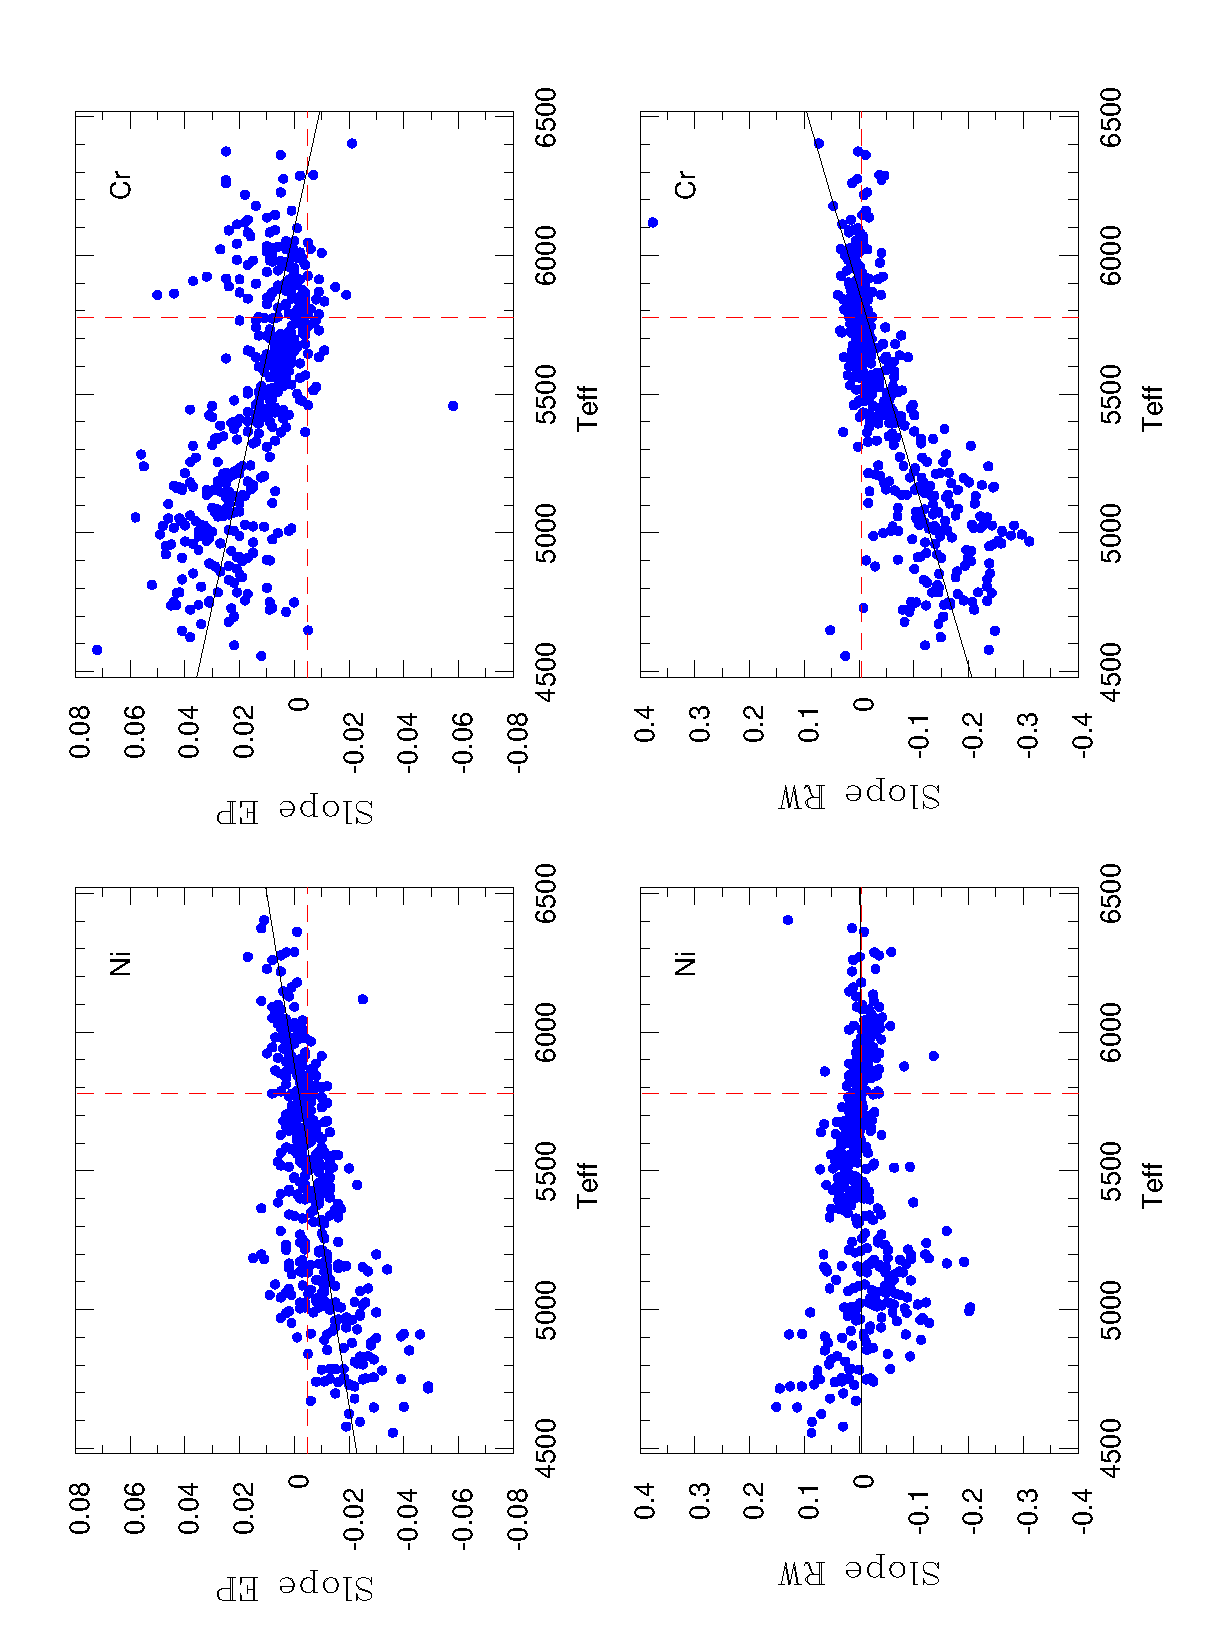
\includegraphics[width= 10 cm, angle=-90]{pics/uncertain/teff.eps}
\caption[Slope EP and slope RW with Teff for Cr and Ni]{Slope EP and slope RW with Teff for Cr and Ni. The red dashed lines mark the solar value. The solid black line represent the linear fit to the points.}
\label{slopeteff}
\end{figure}

\begin{figure}[h]
\centering
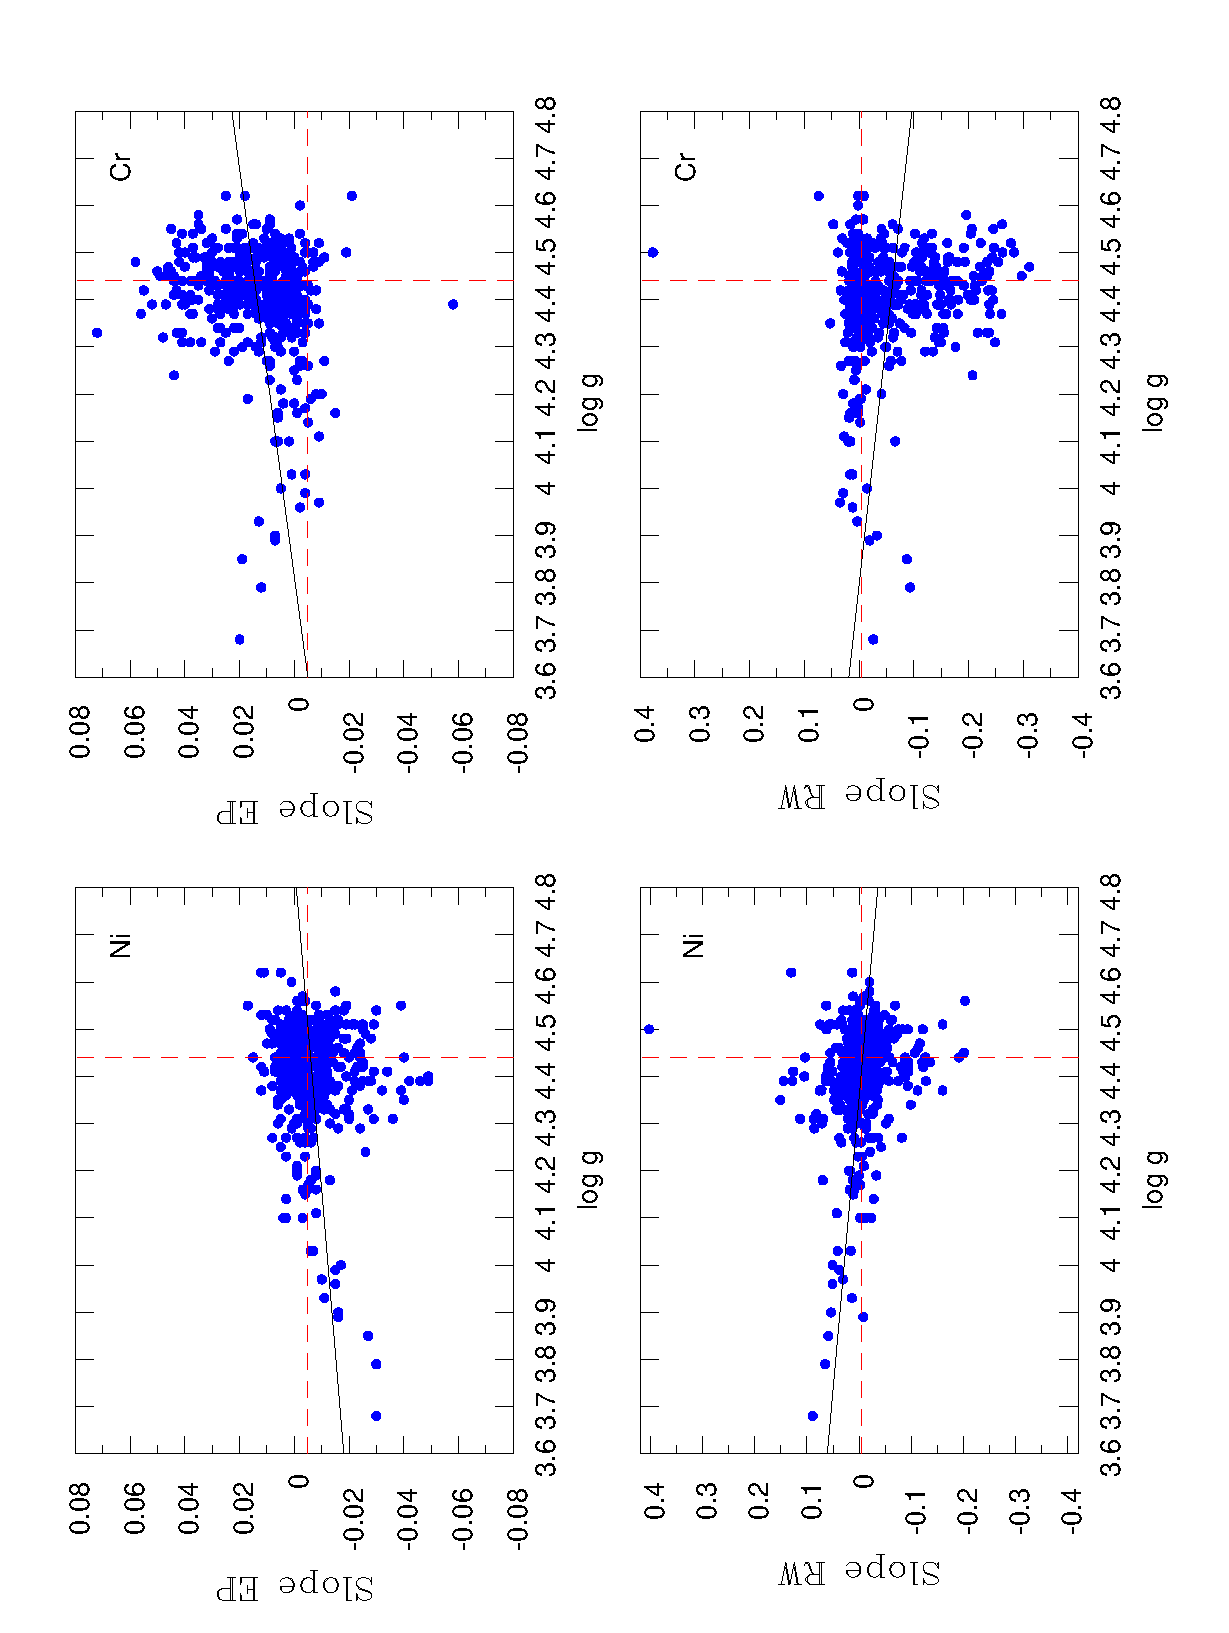
\includegraphics[width=10 cm, angle=-90]{pics/uncertain/logg.eps}
\caption[Slope EP and slope RW with logg for Cr and Ni]{Slope EP and slope RW with surface gravity for Cr and Ni. The red dashed lines mark the solar value. The solid black line represent the linear fit to the points }
\label{slopelogg}
\end{figure}

\begin{figure}[h]
\centering
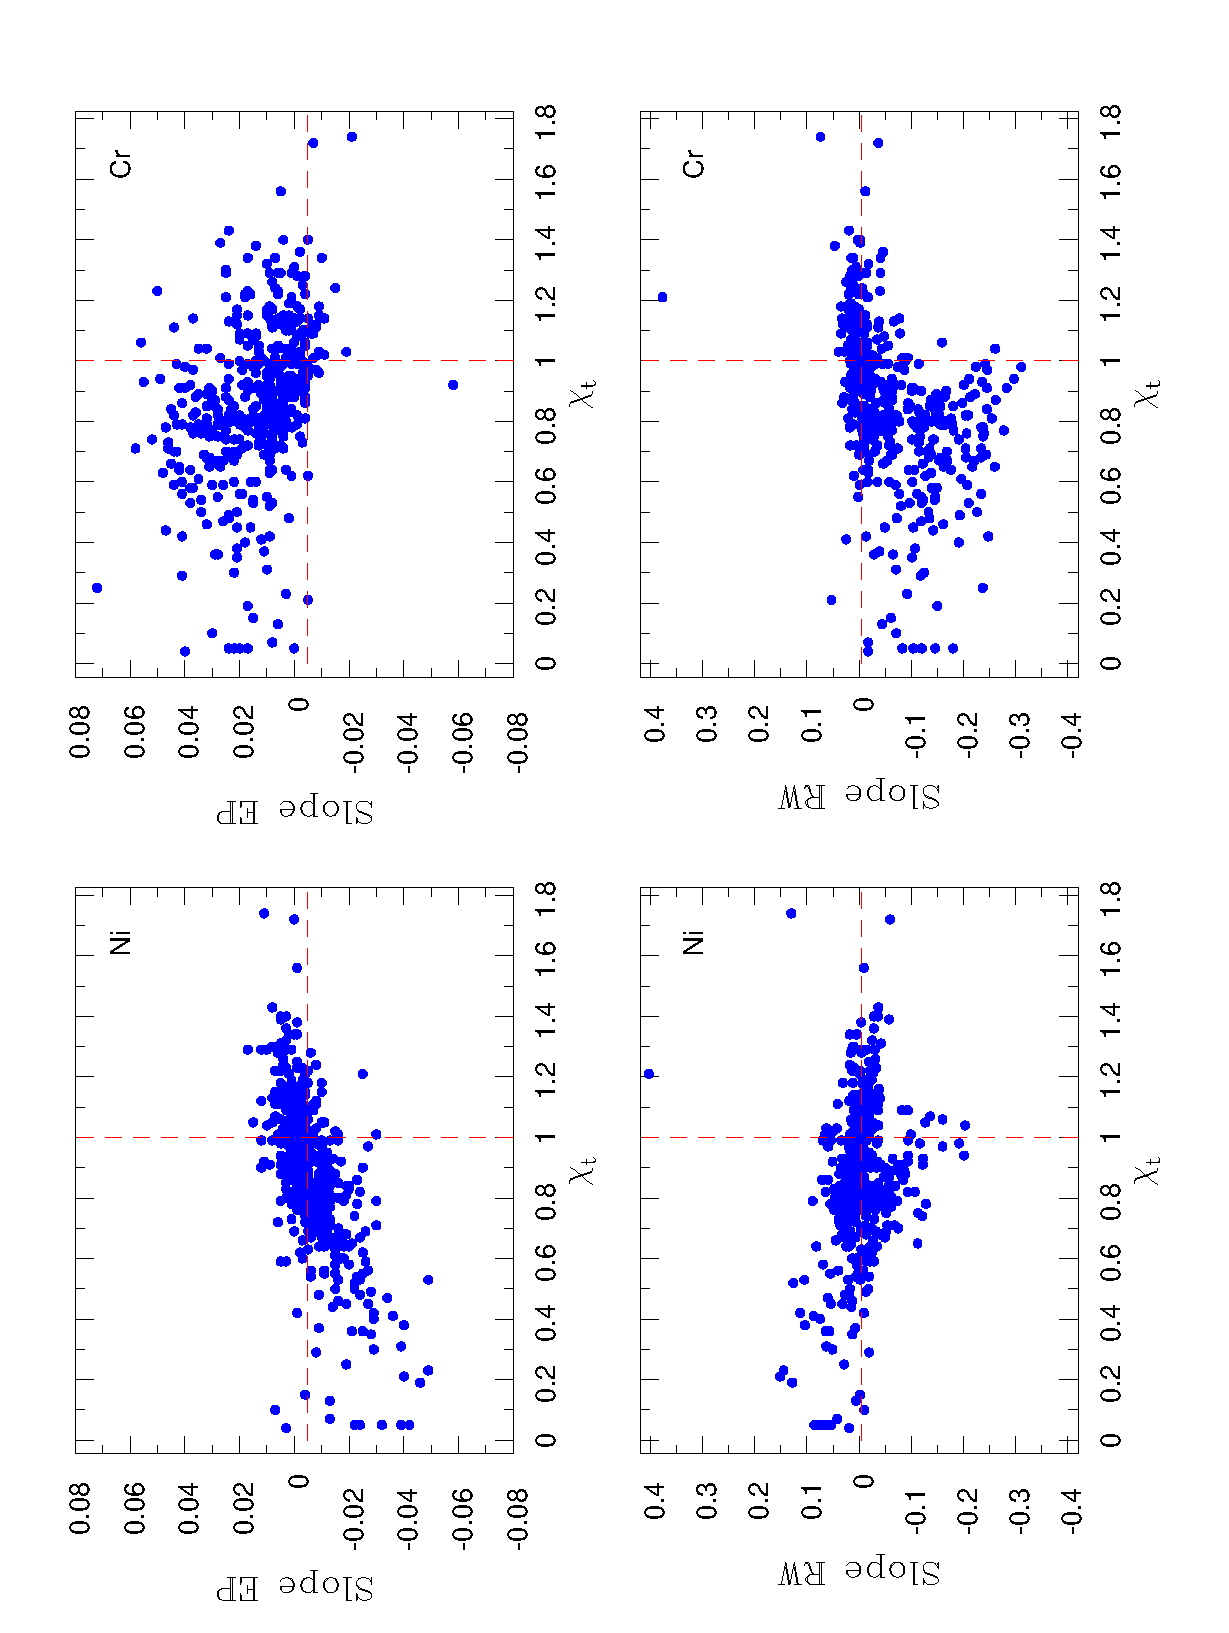
\includegraphics[width=10 cm, angle=-90]{pics/uncertain/vtur.eps}
\caption[Slope EP and slope RW with vtur for Cr and Ni]{Slope EP and slope RW with microturbulence for Cr and Ni. The red dashed lines mark the solar value}
\label{slopevtur}
\end{figure}

\begin{figure}[h]
\centering
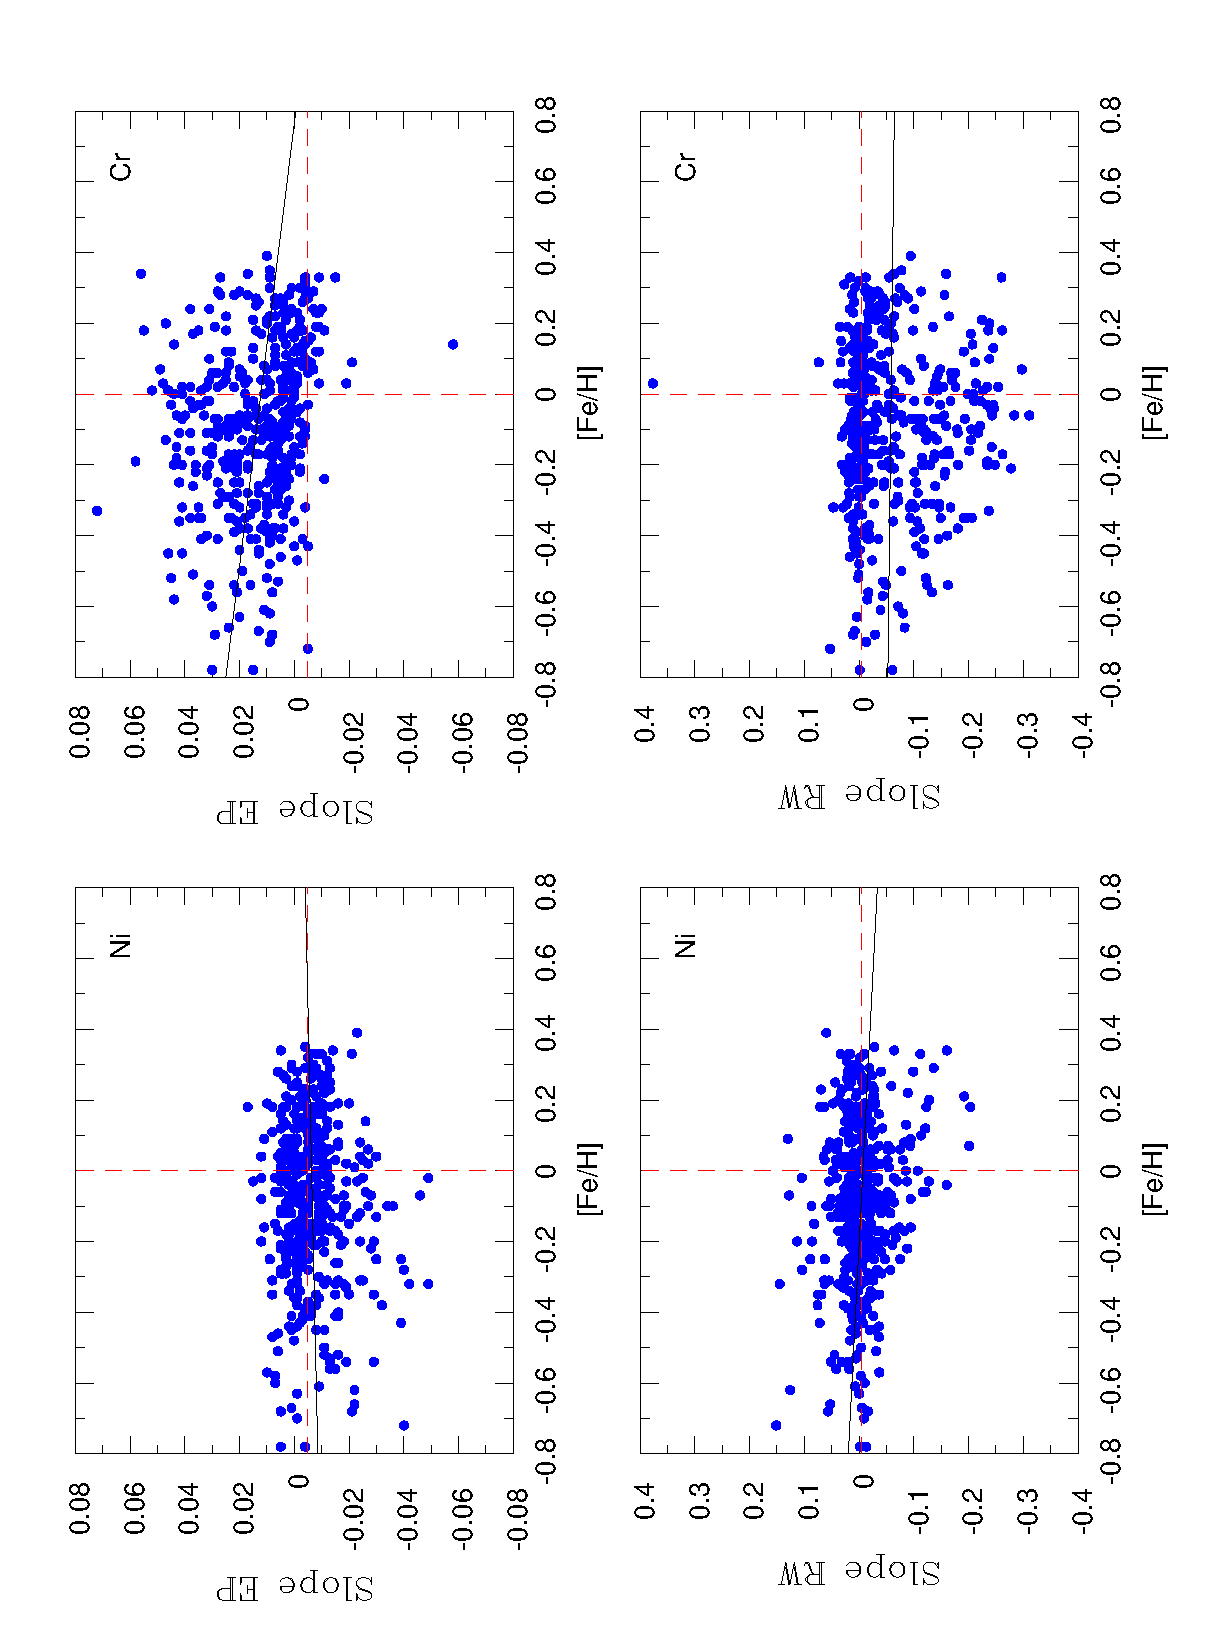
\includegraphics[width=10 cm, angle=-90]{pics/uncertain/feh.eps}
\caption[Slope EP and slope RW with feh for Cr and Ni]{Slope EP and slope RW with metallicty for Cr and Ni. The red dashed lines mark the solar value}
\label{slopefeh}
\end{figure}

From the analysis of the plots, we can't see no discernible trends except in the case of Fig. (\ref{slopeteff}), where we can observe that cooler stars  have more dispersion in average. We can also observe a slight positive slope in Fig (\ref{slopeteff}a) and some unknown trends in the Cr plots for cooler stars, in the same Figure. This might be due to the fact that is much more difficult to measure the EW (due to blending) in cooler stars. We also noted that, in Fig. (\ref{slopeteff}), the Ni dispersion is lower than Cr dispersion for the same plot. The reduced dispersion might be related to the bigger number of Ni lines used to calculate the abundances and/or to the supposed superior quality of the Ni lines. We have also noticed that all the plots of Cr except the one in Fig. (\ref{slopeteff}) show Slope EP having a trend toward positive values and Slope RW having a trend toward negative values. \textcolor{red}{mas porque??? e uma dispersao natural? esta ultima frase esta confusa}


(We also expect that if we plot these slopes in function of the stellar parameters we should also obtain a fit of the data with all slopes approaching the ordinate axis. \textcolor{red}{sera??? mas isto n e para o X/FE? estes slopes sao do X/H!!! precisava de comparar estes gfx com outros - n tenho sensibilidade para ver se aceitavel ou nao. depende da escala! sera q vale a pena fazer fits para estes gfx? - isto temos mesmo q ver pessoalmente})

In another test, we plotted the abundance of every element in function of $T{eff}$ and $log\,g$, represented by Figs. (\ref{xfeteff}) and (\ref{xfelogg}), respectively. We used [X/Fe] to remove the trend of the galactic chemical evolution. The slopes of [X/Fe] as function of the effective temperature per 1000K and as function of the surface gravity can be seen in Table (\ref{slopes}).

\begin{figure}[h]
\centering
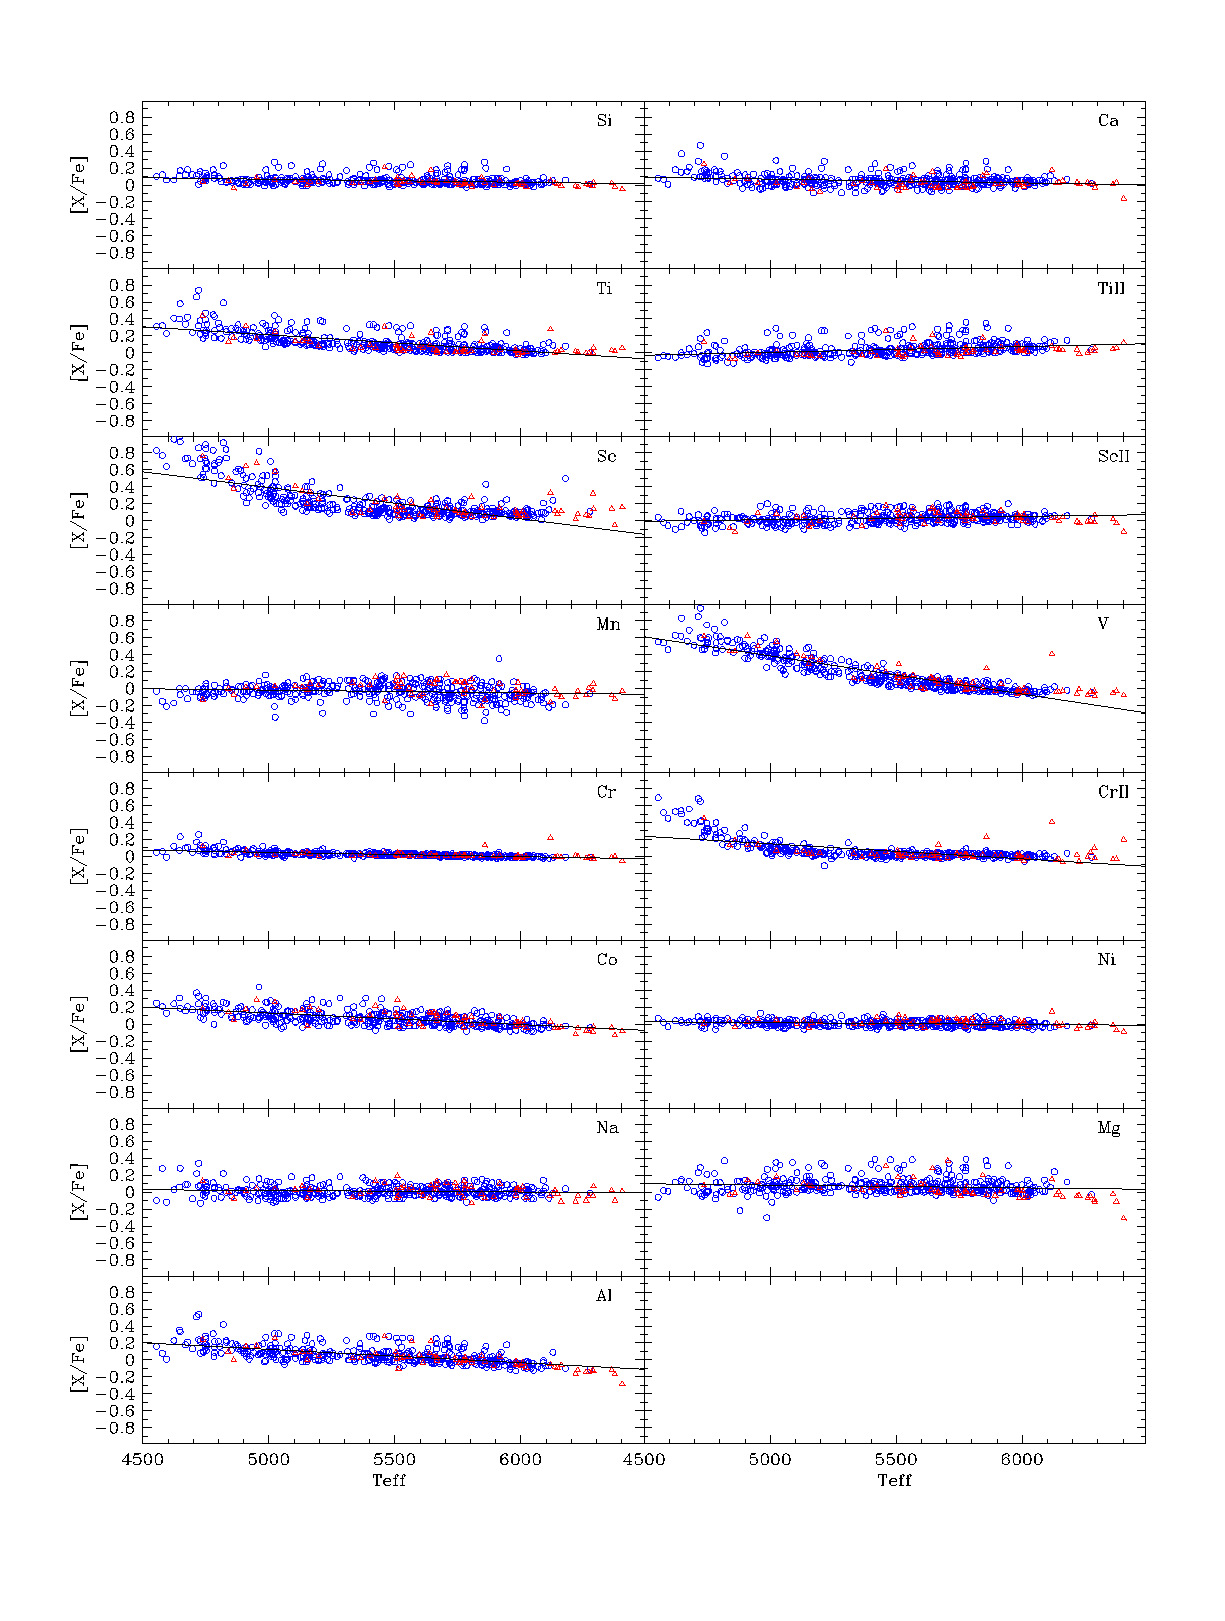
\includegraphics[width=15 cm]{pics/uncertain/xfeteff.eps}
\caption[depois]{[X/Fe] vs. $T_{eff}$. The red triangles are the planet host stars and the blue circles are the stars without planetary companions. Falta meter o solar value. The solid black lines represent the linear fits to both stars.}
\label{xfeteff}
\end{figure}

\begin{figure}[h]
\centering
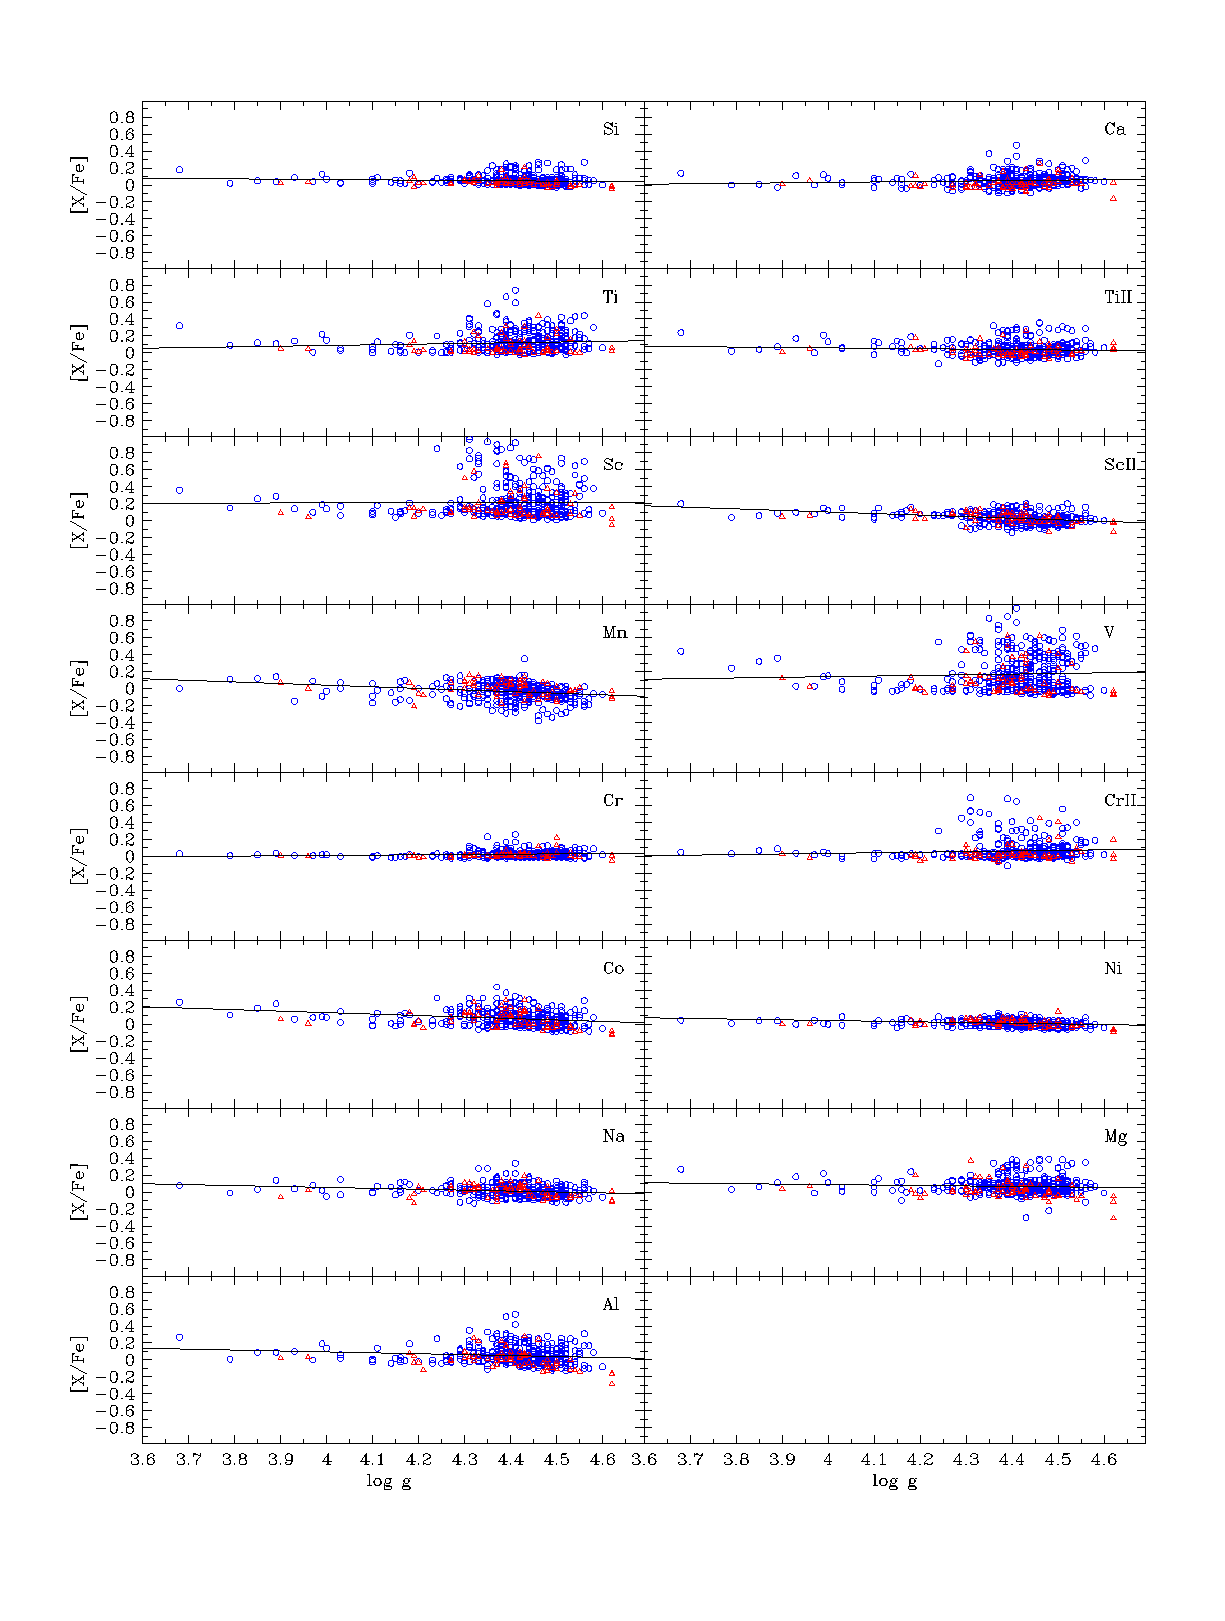
\includegraphics[height=15 cm]{pics/uncertain/xfelogg.eps}
\caption[depois]{[X/Fe] vs. $log\,g$. The red triangles are the planet host stars and the blue circles are the stars without planetary companions. Falta meter o solar value. The solid black lines represent the linear fits to both stars.}
\label{xfelogg}
\end{figure}

\begin{table}[h]
\label {slopes}
\centering
\caption[Slopes of metallicity in function of $T{eff}$ per 1000 K ]{Slopes of $[X/Fe]$ ratio as function of $T_{eff}$ per 1000 K } 
\begin{tabular}{ c r@{$\pm$}l r@{$\pm$}l | c r@{$\pm$}l r@{$\pm$}l}

\hline
\hline 
Species & \multicolumn {2}{c}{$Slope(T)\pm rms$} & \multicolumn {2}{c}{$Slope(g)\pm rms$} & Species & \multicolumn {2}{c}{$Slope(T)\pm rms$} & \multicolumn {2}{c}{$Slope(g)\pm rms$} \\
\hline
Si & -0.036 & 0.051 & -0.037	& 0.053 & Cr & -0.053 &   0.026 & 0.038 & 0.033 \\
Ca &  -0.044 &    0.069 & 0.053 & 0.071 & Cr II &  -0.177 & 0.084 & 0.067 & 0.111 \\
Ti & -0.191 & 0.084 & 0.085	& 0.114 & Co & -0.138 &  0.070 & -0.175 & 0.087 \\ 
Ti II &  0.069 & 0.077 & -0.045 & 0.082 &  Ni & -0.019 & 0.035 & -0.085 & 0.034 \\
Sc & -0.369 & 0.142 & 0.015 & 0.208	& Na &-0.017 &   0.066 & -0.107 & 0.066 \\
Sc II &  0.037 & 0.061 & -0.184 & 0.059 & Mg & -0.033 & 0.096& -0.052 & 0.097 \\
Mn & -0.034  &  0.093  & -0.187 & 0.091 &  Al & -0.159  &    0.080 & -0.111 & 0.102 \\
V & -0.452 & 0.086 & 0.074 & 0.204 \\
\hline

\end{tabular}
\end{table}

We observe significative trends with $T_{eff}$ for Ti I, Sc I, V I, Cr II, Co I and Al I. We can clearly see that the trend away from the expected value,except for Co I and Al I, is heavily influenced by the cooler stars, where the EW might have been overestimated due to blending effects or due to problems associated with the differential analysis: we must not forget that the oscillator strengths were calculated for the Sun. We shall note this bias when we analyze the results. We do not know how to explain the trends observed in Co I and Al I. They might be related to NLTE effects, not taken into account in this analysis.\textcolor{red}{discutir com Nuno}. 

In the case of the $log g$ plots, a clear trend is much more difficult to discern: most stars are in the (4.2 - 4.6) region. Moreover, we verify the existence of a huge dispersion in the same region for Sc, V and Cr II. Despite that, we can see decreasing trends in Sc II, Mn I and Co I. \textcolor{red}{porque sera???}. 

%In order to avoid systematic errors in the measurement of EW due to blending lines or to a poor location in the continuum, we have analyzed the biggest number of lines possible for each element. . 
\textcolor{red}{inda falta meter o gfx da distribuicao da teff do sample e a distribuicao das metalicidades (para mostrar o non bias.}







\appendix

\chapter {The HARPS Spectrograph}
\textcolor{red} isto nao e para ler. esta tudo misturado e n foi revisto...o leitor foi avisado. Se mesmo assim quiser prosseguir, o autor desresponsabiliza-se por todas as consequencias dessa imoral pratica !!!
VER TABLE 1 messenger para dados correctos!!!
\section {Introduction}

In this section we will make a brief discriptions of the technical details, capabilites and ...  of the HARPS spectrograph. For a detailed description of the basic physics, equations and tools behind the operation of a general spectrograph, the prospective reader can consult, for instance, chapter 3 of Gray (2005).

The scientific proposal for HARPS was made in 1999, one year after the decision to build it, following a flurry of exoplanet discoveries that motivated the need for a more potent, precise and dedicated instrument (sci proposal HARPS 1999). The main objective was to reach the 1m/s threshhold for detecting lower mass planets by Radial Velocity with unparalelled accuracy. The HARPS spectrograph was not only made for quality but also for quantity. The observational challenge lied now on observing as many planet host systems as possible in the five year span of the program, in order to have sufficient quality data to do a statistical treatment of all the planetary parameters possible with this technique: distance to host star, minimum mass of the planet, period, excentricity. Moreover, HARPS high spectral resolution (115.000) and S/N ratio has permitted to achieve never seen before spectra of the host stars. From all this data, we hope to reach a better understanding of the physical processes underlying planetary formation. This spectra could also be used to statistically analyse the planet host stars parameters with those of field dwarfs, like, for instance, abundances from several elements, light, volatile and refractory, effective temperatures, spectroscopig $log g$,etc. What are the possible relations among all these parameters, exoplants reserachers asked to HARPS... 

What do we need to achieve these goals? We need a high resolution spectrograph, with a large spectral window, a very stable velocity reference and a fine data reduction process. The technique used to reach this high precision is based on a two fiber fed echelle spectrograph, one fibre for the star and the other iluminating a Thorium-Argon lamp used as reference, allowing the follow up of any instrumental drift. The stellar and reference velocities are calculated by a cross correlation function of both sources. 

\section{limitations}

How can we distinguish the motions of the photosphere due to pulsation and/or stellar activity related to the rotation of star spots or convective inhomogeneities with the motions due to the planets proper? A quantification of these effects can be achieved by comparing the weighted radial velocity dispersion with the typical stellar parameters (spectral type, rotation, magnetic activity) similar to the star being observed. The amplitude of radial velocity variations provoked by instrinsic phenomena may reach some tens of $m/s$ and can therefore inhibit or confuse planet detection. To give an idea, Jupiter's perturbation on the sun velocity is  ~ 12.5 $m/s$.
The present instrumentation accuracy may be limited either by photon noise or by instrumental errors. When aiming at $1m/s$ we must be aware of both sources of errors. 
Considering the photon noise limit, the possible RV precision depends on three factors: the measured flux $S$, the overall spectral resolution $R$ and the observed spectral range $\lambda\lambda$, according to Hatzes and Cochran 1992 (n consigo encontrar artigo!!! 
\begin{equation}
\frac{1}{\sigma v_r}\propto S^{0.5}\lambda^{0.5}R^{1.5}
\end{equation}
The best way to increase the RV precision is to increase as much as possible the resolution of the spectrograph. Unfortunately this leads to large instrument size, without the use of adaptative optics or image slicers, which were not adequate to HARPS. The solution was to install the largest echelle grating possible. The ideia was to increase the resolution to the point where the stellar spectral lines start to be resolved. The comprimise for $R$ was set at ~ 100.000. Even at this high resolution, slit losses remain below 50\%. 

\section{Comparing HARPS with other spectrographs}
How does HARPS spectrograph fare agains other similar instruments? In the following table, we can observe a comparison table of instrument overall eficiencies. The coefficient $Q_{night}/Q_{HARPS}$ represents the efficiency of the instrument to reach a given photon-noise precision per observing night, compared to HARPS, taking into account the telescope size, the spectral bandwidth, resolution and transmission differences between the spectrographs. The technique is ThAr lamp if the number of fibers are shown. Otherwise it's the Iodine Technique. $Q_{year}/Q_{HARPS}$ corresponds to the same value integrated over 1 year, taking into account the time allocation for planet search only. 

As we can see, HARPS is superior to every instrument on the table, exept the VLT UVES with the FLAMES link due to its multi fibre configuration. The HARPS supremacy is even greater if we take into account the efficiency coeficient per year that includes telescope time for planet search of each instrument. 

The improvement in the precision of RV measurments from 5-10 $m/s$ down to 1 $m/s$, will largely contribute to remove biases in the detection of extra solar planets.  This will permit the detection of very light giant planets only with one tenth of the mass of saturn, although terrestrial planets should be out of reach if the 1 $m/s$ limits apply throughout the lifetime of the instrument (obviamente que nao). -- ver figura 8 se n tiver noutro sitio. 

\section{Instument Overview}

HARPS stands for \textbf{H}igh \textbf{A}ccuracy \textbf{R}adio \textbf{V}elocity \textbf{P}lanetary \textbf{S}earcher and is an instrument designed to measure high precision and high resolution Radial Velocities (RV). Its main goal is to reach a RV accuracy of 1 $m/s$ for slowly rotating solar type stars. This never before reached precisions enable the detection of low mass extra solar planets (a little smaller than Saturn). 
The design of HARPS was based on previous observational programs like ELODIE and CORALIE during the past 10 years. The basic design of HARPS is very similar to these. The main advantages of HARPS are as following:
\begin{itemize}
 \item Greater instrument stability. The spectrograph is installed in a sealed and evacuated enclosure with low temperature. This almost completely eliminates drifts in RV due to temperature, pressure or humidity variations.
\item Increase of S/N. The 3.6m ESA telescope on witch HARPS is installed is bigger than it's predecessors. Therefore, the S/N ratio is better. Moreover, the resolution of the CCD is increased by a factor of two and this also permits to reduce intrumental errors.
\item Improvement of online data reduction. includes better corrections for instrumental effects and is faster.
\end{itemize}

HARPS is a fibre-fed, cross dispersed echelle spectrograph. It operates at 17$^o$C constant within  0.005$^oC$ RMS, with a pressure < 10$^{-2}mbar$. It is located in the Coude' floor of the 3.6m telescope. 
Two fibers, an object and a reference fibre fed the spectrograph with light from the telescope and from the calibration lamps. The light is reimaged by the internal optics onto a mosaic of two 2k4 CCDs were two spectra of 72 orders are formed. The spectral region goes from 380 to 690nm. At the resolution of 115.000 each spectral element is sampled by 3.2 CCD pixels. A summary of the specs are shown below (messenger 114). 
The optics are mounted on a 2.5m optical bench made of plated steel. The spectrograph has no moving parts and is located inside a vaccum vessel in a thermally stabilized enclosure.  
The illumination is critical for RV precision. This is guaranteed thanks to the light scrambling properties if the optic fibres. 
HARPS is an ordinary spectrograph. However it distinguishes itself mainly by his incredible stability:The ThAr reference is able to detect even the tiniest of instrumental drifts. Nevertheless lots of efforts was put into place to make HARPS intrinsically stable, in order to avoid any kind of second order intrumental errors. Consequently, the spectrograph operates in low vacuum since pressure variations may produce huge drifts in the order of 100m/s per mbar. The pressure was put under $10^{-2}$ mbar so that the drifts do not exceed 1m/s per day. Temperature was also controlled...When the instrumental noise produced by the thermal dilatation of the CCDs due to tiny temperature variations is removed we get dispersion values consistent with photon noise of the ThAr reference lamp. This technique can track drift variations at 0.1 $m/s$. Factors like resolution, optical efficiency, size of instrument and telescope, fiber diameter, must be balanced in order to have the smallest instrumental errors. 
After several tests, the attained value for the HARPS precision was well below 1 $m/s$. Even on the time scale of a comission (2 weeks) we could obtain values of dispersion no greater than 1 m/s. This same level of precision was obtained even in surveys with a timescale over 4 months. At this precision level, we must count that one of the most probable sources of dispersion is the star itself (pulsations, activity, jitter). 
The data analysis of all the accumulated observations are still being done in order to determine  which effects are limiting the precision of RV measurements. Disentangling noise and systematics from instrumental and stellar origin in not a trivial task. It needs time and lots of data. This will be very important for the preparation of the next generation instruments like CODEX on OWL telescope. 
The best residuals obtained are as low as 0.2 m/s which indicates that with enough observations, it will be possible to detect a 3 $M_\oplus$at 1 AU. But it seems reasonable that it is possible to average out most of the perturbing effects (stellar oscilations, activity jittering...). when observing in timescales compared to the periods of these effects. 
Efforts in the improvement of calibration with the ThAr lamps using a new HARPS made atlas with very high resolutions has enabled to reach new global uncertainties in the calibration  (RV zero point) from 0.8 m/s to 0.2-0.4 m/s. 

\section{Other error sources}

The most obvious error source is photon noise: it is the one coming from the finite number of photons collected in a stellar spectrum. The fundamental uncertainty on the RV depends both on the number of recorded photons and on the intrinsic slope of the spectrum. 
Guiding noise is the noise that originates from changes in the fibre illumination. This is very critical. This can cause spurious RV variations. With proper software to monitor the centering of the fibre at the middle of the stellar image the guiding noise contributes no more than 0.3 m/s to the global dispersion.
Stellar Oscilation Noise. Solar type stars show p mode oscilations with periods of a few minutes and amplitudes of a few m/s. However some of these signals can superimpose. The present strategy regarding this noise is to integrate over a few characteristic periods to average out these effets as much as possible. This maintains this noise below 1 m/s.
Stellar activity related jitter. Magnetic phenomena at the surface of solar type stars can induce RV perturbations in the order of 100 m/s. This prevents completely the use of RV tequenique to detect planetary companions. Stars in the HARPS catalogue are chosen for showing low chromospheric activity and slow rotation. to ensure that these effects stay below a few m/s. Hopefully, the binning of data points over the stellar rotation will permit to average out these effects, but this is still on an experimental phase.






\section{The Telescope}
The ESO La Silla 3.6m telescope, home of the HARPS spectrograph, is equatorially mounted. HARPS use the Cassegrain focus. A general discription of the telescope can be found here: http:\\www.ls.eso.org/lasilla/sciops/3p6/. 

\section{Spectrograph}

The Vaccum vessel protects the spectrograph proper from variations in temperature, pressure and humidity. Is is evacuated by a turbo molecular pump before the start of operations. The vaccum is regenerated once or twice per month. 

The Spectograph itself is a cross dispersed echelle spectrograph, similar to UVES @ VLT. The echelle grating is operated in a quasi Littrow operation (ver). An f/2.1 parabolic mirror serves as collimator. A dioptric camera images the cross dispersed spectra side by side onto a mosaic of two 2kx4k EEV CCDs. The spectral range goes from 378 to 691 nm. All components are mounted on a stainless steel optical bench. The optical paremeters of HARPs are those of Table X.X.

\section{Detector System}

Harps employ a mosaic of two EEV type 44-82 CCDs. The spectral format is 4096x4096 pixels. Its properties are summarized in the following table. 

\section {Calibration Unit}

It provides the instrument with light for wavelength and flatfield calibration. This calibration is based on a set of Thorium-Argon and halogen lamps. The calibration fibre pair connects the calibration unit with the fibre adapter at the Cassegrain focus. 

\section {Data reduction}

The data reduction pipeline is a software developed by ESA which allows the reduction of the spectra in almost real time. 


Both stray light and ghosts are present at some level, most noticeable in the blue part of the spectrum. This is due to the fabrication process of the grid itself (defects). The characteristic optical data of HARPS can be seen in Table X.X.


















%------------------------------------------------------------------------------------------------------------------------------------------------------
%------------------------------------------------------------------------------------------------------------------------------------------------------
\newpage
%\addcontentsline{toc}{chapter}{Bibliography}
%\bibliographystyle{plainnat}
%\bibliography{report}

%\newpage
%\addcontentsline{toc}{chapter}{\numberline{ }List of Figures}
%\listoffigures
%\newpage
%
%\newpage
%\addcontentsline{toc}{chapter}{\numberline{ }List of Tables}
%\listoftables
%\newpage

%\addcontentsline{toc}{chapter}{\numberline{ }Anexos}
%\bibliographystyle{plain}
%\bibliography{mylib}


\bibliographystyle{aa}
\bibliography{mylib}


\end{document} 

%FIGURAS%%%%%%%%%%%%%%%%%%%%%%%
%%%%%%%%%%%%%%%%%%%%%%%%%%%%%%%
\begin{figure}[h]
\begin{center}$
\begin{array}{cc}
\includegraphics[scale=0.25]{figs/} &
\includegraphics[scale=0.25]{neptune_v16_1_100_10d6_exc_PT_1930PL.eps}
\end{array}$
\end{center}
\caption[Varia��o da excentricidade de Plut�o.]{Gr�fico da varia��o da excentricidade de Plut�o ao longo do tempo. A imagem da esquerda foi obtida para 300 mil anos e a imagem da direita para 10 milh�es de anos. A excentricidade m�dia � $\bar{e_1} \sim 0.24$.} \label{fig:exc1930PL}
\end{figure}
